<<<<<<< HEAD
\chapter{Opis implementacji}
\label{cha:Opis implementacji}
\section{Zastosowana platforma sprzętowa}
\label{sec:Zastosowana platforma sprzętowa}
Zdecydowano się na płytkę rozwojową Digilent~Zybo~Z7-20 oraz~kamerę~Digilent PCAM~5C. Przeprowadzenie syntezy i~implementacji możliwe było przy użyciu darmowego oprogramowania Vivado SDK WebPack. Podczas prac używano wersji~2018.2. Płytka wyposażona była w układ FPGA XC7Z020-1CLG400C stanowiący część rekonfigurowalną (PL -- ang. \textit{programmable logic}) oraz dwurdzeniowy procesor Cortex-A9 (PS -- ang. \textit{processing system}), taktowany z~częstotliwością 667~MHz. Oba komponenty zostały wykorzystane w projekcie. Do dyspozycji projektanta pozostawało 53 200 tablic LUT (ang. \textit{Look-up Table}), 106 400 przerzutników \textit{flip-flop} oraz 630 KB pamięci blokowej RAM. \\
Producent na swojej stronie internetowej zapewnia projekt demonstracyjny połączenia kamery i~płytki~\cite{projektPCAM}. Przez port szeregowy możliwa jest zmiana rozdzielczości, szybkości akwizycji ramek, współczynnika korekcji gamma, ustawień balansu bieli. Możliwe są następujące opcje dotyczące dwóch pierwszych parametrów:
\begin{itemize}
	\item 1280 x 720, 60 fps,
	\item 1920 x 1080, 15 fps,
	\item 1920 x 1080, 30 fps.
\end{itemize}
Testy pokazały również, że dla rozdzielczości 1280 x 720 większy jest kąt widzenia kamery. Kwestię tę opisano w~sekcji \ref{sec:wyznaczenia_kata_kamery}. Ze~względu na~powyższy fakt oraz przyspieszenie obliczeń, zdecydowano się na~najmniejszą dostępną rozdzielczość.\\
Pobrany projekt stanowił bazę do dalszych prac. 
\section{Implementacja modelu programowego}
\label{sec:Implementacja modelu programowego}
Model programowy został napisany w pakiecie Matlab przy wykorzystaniu funkcji dostępnych w~Image Processing Toolbox. Pozwoliło to na sprawne wykonywanie operacji na~obrazach.
Aby możliwe było wprowadzanie ramek obrazu do modelu, należało umożliwić akwizycję obrazów na kartę SD. Uaktywniono interfejs procesora SD0, do~projektu w~SDK dodano bibliotekę ,,xilffs'' i,~korzystając z~funkcji systemu plików opisanych w~\cite{xilffs}, napisano zapis ramek do~pliku. Ze~względu na~prostotę pliku, składającego się jedynie z~nagłówka oraz wartości kolejnych składowych RGB, zdecydowano się na format ppm.\\
W~późniejszym stadium projektu, z~powodu różnic na obrazie zapisywanym na ramkę i~wyświetlanym na ekranie, zdecydowano się na zmianę tej koncepcji. Zaimplementowano cały tor wizyjny w~części PL układu Zybo Z7-20 i~przechwytywano przetworzone obrazy wyświetlane na~monitorze. Dzięki takiemu podejściu podczas testowania widziano rzeczywiste wyniki przetwarzania.
\section{Implementacja toru wizyjnego w układzie}
\label{sec:impl_tor_wizyjny}
\subsection{Konwersja z przestrzeni barw RGB do YCbCr}
\label{subsec:konwersja}
Przestrzeń barw YCbCr wykorzystuje 3~zmienne: składową luminancji Y, składową różnicową chrominancji Cb, która wyraża różnicę między luminancją, a niebieskim, oraz składową różnicową chrominancji Cr, oznaczającą różnicę między luminancją,~a~czerwonym. Zaletą stosowania tej przestrzeni barw jest oddzielenie sygnału luminancji od~sygnałów chrominancji, pozwalające na~dokonywanie dalszej obróbki sygnału przy mniejszej zależności od~oświetlenia.
Konwersję z przestrzeni barw RGB do YCbCr wykonano zgodnie ze wzorem \ref{eq:ycbcr}. Przy implementacji wykorzystano sprzętowe mnożarki oraz sumatory.
\begin{equation}
\label{eq:ycbcr}
\begin{bmatrix} Y \\ 
				Cb\\
				Cr
\end{bmatrix}=
\begin{bmatrix} 0,299 & 0,587 & 0,114\\ 
				-0,168736 & -0,331264 & 0,5\\
				0,5 & -0,418688 & 0,081312
\end{bmatrix}
\begin{bmatrix} R\\
				G\\
				B
\end{bmatrix}+
\begin{bmatrix} 0\\
				128\\
				128
\end{bmatrix}
\end{equation}
\subsection{Binaryzacja}
\label{subsec:Binaryzacja}
% dobieranie progu: 2 multiplekser sterowany buttonem?
Piksel wyjściowy otrzymywał wartość maksymalną (kolor biały), jeśli wartości Cb i~Cr mieściły się pomiędzy wyznaczonymi eksperymentalnie progami. W~innym przypadku pikselowi przypisywana była wartość 0 (kolor czarny). Moduł binaryzacji pracował z zerową latencją.
\subsection{Mediana}
\label{subsec:Mediana}
% obrazek wyznaczania kontekstu
% obrazek drzewa sumacyjnego
Mediana to operacja kontekstowa, w~której pikselowi wyjściowemu przypisuje się wartość środkową uporządkowanego zbioru wartości pikseli z~otoczenia piksela wejściowego. W~przypadku działania na~obrazie binarnym operacja taka może być przeprowadzona przez obliczenie sumy wartości pikseli kontekstu, a~następnie porównanie jej z~połową maksymalnej wartości tej sumy. Ze względu na łatwość implementacji oraz wystarczające działanie, zdecydowano się na~rozpatrywanie kontekstu w~kształcie kwadratu o~boku 5~pikseli. Spowodowało to~konieczność zapamiętywania kontekstu piksela w~25 rejestrach oraz 4~linii obrazu w długich liniach opóźniających zbudowanych w~oparciu o~pamięć BRAM. Schemat wyznaczania kontekstu przedstawiono na rysunku \ref{fig:kontekst}. Sygnały synchronizacji zostały doklejone do wartości piksela i~w~przedstawionej strukturze przesuwają się razem z~nim. Sumę wyliczano w~2~etapach, dodając najpierw elementy w~wierszach, potem sumując wyniki. Latencja modułu wynosiła 2, należało zatem opóźnić sygnały synchronizacji o~tyle taktów zegara.
\begin{figure}[h]
	\centering
	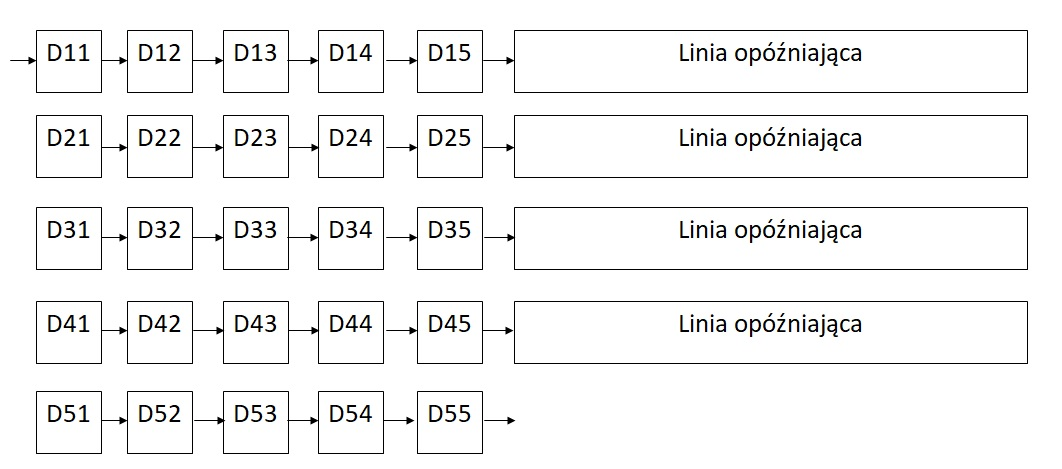
\includegraphics[width=\textwidth]{kontekst.jpg}
	\caption{Schemat wyznaczania kontekstu dla mediany, erozji i dylatacji.}
	\label{fig:kontekst}
\end{figure}  
\subsection{Erozja i dylatacja}
\label{subsec:Erozja}
Erozja i dylatacja to~operacje morfologiczne, w~których pikselowi wyjściowemu przypisuje się wartość odpowiednio najmniejszego i~największego piksela w~sąsiedztwie piksela wejściowego. Sąsiedztwo piksela określa kształt i~rozmiar elementu strukturalnego. Podobnie jak w~przypadku mediany, zdecydowano się na~kwadrat o~boku 5~pikseli. Moduł erozji ustawia wartość piksela wyjściowego na~maksymalną wartość, gdy~w~sąsiadztwie znajdują się same białe piksele. W~module dylatacji zwracana jest wartość maksymalna, gdy przynajmniej jeden piksel w~sąsiedztwie ma kolor biały. Latencja modułów wynosi~1.
\subsection{Środek ciężości i prostokąt otaczający}
\label{subsec:Środek ciężości}
\noindent Wyznaczając środek ciężkości pikseli należących do~obiektu, wykorzystano wzory \ref{eq:m00}, \ref{eq:m10} i~\ref{eq:m01}.
\begin{equation}
\label{eq:m00}
m_{00}=\sum_{i=0}^{N-1}\sum_{j=0}^{M-1} x_{ij}
\end{equation}
\begin{equation}
\label{eq:m10}
m_{10}=\sum_{i=0}^{N-1}\sum_{j=0}^{M-1} i*x_{ij}
\end{equation}
\begin{equation}
\label{eq:m01}
m_{01}=\sum_{i=0}^{N-1}\sum_{j=0}^{M-1} j*x_{ij}
\end{equation}
gdzie:
\begin{eqwhere}[2cm]
	\item[$N$] szerokość obrazu w pikselach,
	\item[$M$] wysokość obrazu w pikselach,
	\item[$x_{ij}$] wartość piksela o~współrzędnych i, j obrazu zbinaryzowanego.
\end{eqwhere}
Na ich podstawie obliczono środek ciężkości przy zastosowaniu wzorów \ref{eq:xsc} i~\ref{eq:ysc}.
\begin{equation}
\label{eq:xsc}
X_{sc}=\frac{m_{10}}{m_{00}}
\end{equation}
\begin{equation}
\label{eq:ysc}
Y_{sc}=\frac{m_{01}}{m_{00}}
\end{equation}
\begin{eqwhere}[2cm]
	\item[$X_{sc}$] współrzędna pozioma środka ciężkości,
	\item[$Y_{sc}$] współrzędna pionowa środka ciężkości.
\end{eqwhere}
W~module na podstawie sygnałów synchronizacji oraz wymiarów obrazka wyznaczono współrzędne aktualnie przetwarzanego piksela. Jeśli jest to piksel należący do obiektu, następuje zwiększenie wartości odpowiednich rejestrów zgodnie ze wzorami
\ref{eq:m00}, \ref{eq:m10} i~\ref{eq:m01}. Po przejściu przez całą ramkę obrazu wykonywane jest dzielenie na podstawie wzorów \ref{eq:xsc} i~\ref{eq:ysc}.\\
W module zintegrowano wyznaczanie środka ciężkości oraz prostokąta otaczającego. Znalezienie prostokąta sprowadza się do wyznaczenia skrajnych jego punktów na górze, dole, po lewej oraz prawej stronie. Do odpowiednich rejestrów trafiają wartości współrzędnych piksela, jeśli wykraczają poza aktualną zawartość rejestrów.\\
Moduł zwraca wartości współrzędnych środka ciężkości oraz skrajnych punktów prostokąta otaczającego.
\subsection{Indeksacja}
\label{subsec:Indeksacja}
Indeksacja to operacja pozwalająca na wydobycie z~obrazu poszczególnych obiektów. Obiekty rozumiane są jako grupy połączonych ze sobą pikseli. Zazwyczaj na wejście modułu indeksacji podawany jest obraz zbinaryzowany, natomiast na~wyjściu pojawia się ramka z~pikselami, których wartość odpowiada przypisanej do~danego obiektu etykiecie. Rozważane jest otoczenie każdego piksela, składające się z trzech pikseli nad nim oraz jednego po~lewej stronie, tak jak zostało to przedstawione na rysunku \ref{fig:ind_sasiedztwo}. Indeksacji dokonuje się bezpośrednio na~obrazie wejściowym. Podczas iteracji po wszystkich pikselach, w~przypadku znalezienia piksela należącego do któregoś z~obiektów, może zajść jeden z~trzech przypadków:
\begin{enumerate}[label=(\alph*)]
	\item w otoczeniu piksela znajdują się same piksele nienależące do~żadnego obiektu,
	\item otoczenie zawiera jeden lub więcej pikseli, którym została wcześniej przypisana taka sama etykieta~L,
	\item w otoczeniu znajdują się piksele posiadające różne etykiety.
\end{enumerate} 
\begin{figure}[h]
	\centering
	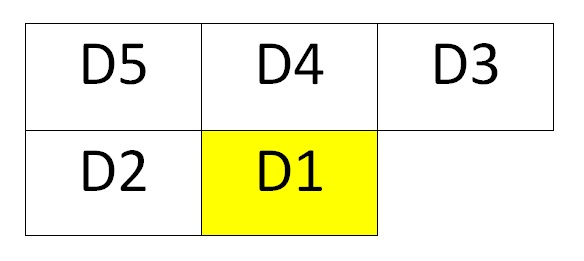
\includegraphics[width=\textwidth]{ind_sasiedztwo.jpg}
	\caption{Sąsiedztwo piksela brane pod uwagę przy indeksacji}
	\label{fig:ind_sasiedztwo}
\end{figure}
W~pierwszym przypadku pikselowi zostaje przypisana nowa etykieta. Gdy spełniony jest warunek b, punkt otrzymuje etykietę L, natomiast jeśli zachodzi przypadek c, przypisywana jest mniejsza z~etykiet. W~ten sposób otrzymuje się obraz wstępnie poetykietowany. Najczęściej posiada on więcej przypisanych etykiet, niż obiektów. Dlatego istnieje konieczność złączenia ze~sobą pewnych etykiet przy użyciu tablicy sklejeń. Tablica ta zawiera informację, które etykiety powinny zostać złączone. W~przypadku~a do tablicy sklejeń na~pozycji odpowiadającej etykiecie zapisywana jest etykieta, natomiast gdy zachodzi opcja~c etykietę mniejszą zapisuje się pod indeksem większej. Do sklejenia etykiet potrzebna jest druga iteracja, tym razem po~obrazie wstępnie poetykietowanym.\\
Powyższy fakt jest główną przeszkodą w~łatwym wykonaniu takiego algorytmu w~systemie potokowym. Bez~zapamiętywania całej ramki, w~przypadku sklejania etykiet, niemożliwy jest powrót do~wcześniej przetwarzanych pikseli. Pomimo tego, możliwe jest obliczenie pewnych cech obiektów, takich jak: pole, współrzędne środka ciężkości, prostokąt otaczający. W~pracy \cite{COG} podano sposób, w~jaki można tego dokonać. Opiera się on~na~scaleniu nie samych wartości pikseli, ale~obliczanych na~bieżąco parametrów obiektu.\\ Implementacja w~języku Verilog rodzi dodatkowo trudności związane z~określeniem przypadku istnienia tej~samej lub~różnych etykiet w~otoczeniu piksela. Utrudnienie stanowi brak możliwości wykorzystania funkcji eliminującej zera z~wektora, czy znajdującej minimum i~maksimum. O~ile~zachodzenie przypadku a jest łatwe do wykrycia, to~przypadki b~i~c wymagały rozważenia kilku możliwości. Zdecydowano się na~wykrywanie ich za~pomocą flag bitowych. Na~ich podstawie wnioskowano o~zachodzącym aktualnie przypadku oraz wskazywano, od~którego piksela z~otoczenia powinna zostać przepisana etykieta. Oprócz tego, na bieżąco obliczano prostokąt otaczający oraz liczbę pikseli należących do~każdego ze~znalezionych obiektów.\\
Po poetykietowaniu całej ramki obrazu wykorzystano tablicę sklejeń do~złączenia obliczanych na~bieżąco cech. Ten~etap algorytmu zaimplementowano jako maszynę stanów:
\begin{itemize}
	\item Stan 0 -- Oczekiwanie na sygnał końca ramki wyznaczany na podstawie synchronizacji pionowej. W~momencie wykrycia sygnału następuje rejestrowanie tablicy sklejeń i~obliczonych parametrów, zerowanie tablic wypełnianych w~kolejnym etapie oraz przejście do~stanu~1.
	\item Stan 1 -- Iteracja po tablicy sklejeń i~uzupełnianie rzeczywistych wartości cech obiektów.
	\item Stan 2 -- Uporządkowanie tablic z~wyznaczonymi parametrami.
	\item Stan 3 -- Obliczenie pola prostokąta otaczającego dla każdego znalezionego obiektu. Wykorzystywana jest mnożarka o~latencji 3.
	\item Stan 4 -- Szukanie obiektu spełniającego warunki minimalnej wielkości pola powierzchni oraz stosunku pola prostokąta otaczającego do pola obiektu. W~przypadku znalezienia takiego kształtu, na~wyjście trafiają współrzędne jego prostokąta otaczającego. Jeśli żądany kształt nie zostanie znaleziony, informacja o~tym również pojawi się na~wyjściu.
\end{itemize}
Schemat przetwarzania danych po~każdej ramce pokazano na rysunku \ref{fig:ind_schemat}
\begin{figure}[h]
	\centering
	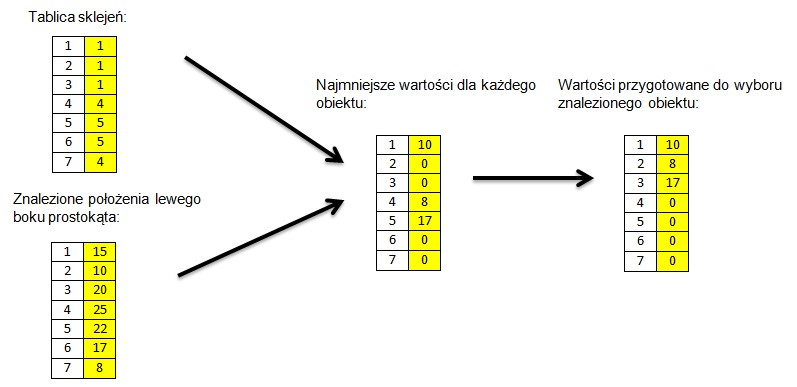
\includegraphics[width=\textwidth]{ind_schemat.jpg}
	\caption{Schemat procesu przetwarzania informacji po~każdej ramce obrazu z przykładowymi danymi.}
	\label{fig:ind_schemat}
\end{figure}
\\Główną trudnością w~implementacji opisanego algorytmu w~układzie FPGA jest stosunkowo duze zapotrzebowanie na~zasoby sprzętowe. Należy zarezerwować miejsce na~cechy każdego potencjalnego obiektu. Ogranicza to~liczbę możliwych etykiet. Zarezerwowanie miejsca dla 30~obiektów nie~przekroczyło możliwości układu Zybo. Badania pokazały, że~jest to wystarczająca liczba etykiet do~sprawnego działania toru wizyjnego.
\section{Komunikacja układu ZYBO Z7-20 ze sterownikiem Pixhawk}
\label{sec:komunikacja_pixhawk} 
--- Tutaj chciałbym opisać protokół Mavlink używany do komunikacji ze sterownikiem. Obecnie została nawiązana komunikacja i udało się wysłać komendę uzbrojenia drona w trybie STABILIZE. W najbliższym czasie planuję przeprowadzić test wysyłania komend ruchu w trybie GUIDED, który wymaga połączenia GPS.
%-------------------------------------------------------------------------
=======
\chapter{Implementacja i ewaluacja modelu programowego}
\label{cha:opis_implementacji}

%TODO2 Modyfikacja opisu
W~rozdziale szczegóły związane z~implementacją systemu. 
Ważną rolę w~tworzeniu kolejnych modułów odegrał model programowy, czyli program napisany w~dowolnym języku programowania i~wykonywany na~komputerze~PC, którego działanie oddaje funkcjonalność modułu tworzonego w~sprzęcie.
Porównanie wyników działania modelu programowego i~symulacji modułu daje informację o~poprawności implementacji. 
Model programowy, wraz z~uzasadnieniem użycia poszczególnych modułów, przedstawiono na~początku rozdziału.
Następnie opisano wszystkie wykonane komponenty, od~przesłania obrazu przez kamerę, do~wysyłania komend do~autopilota.

\section{????}
\label{sec:implementacja_modelu_programowego}
Model programowy został napisany w pakiecie Matlab przy wykorzystaniu funkcji dostępnych w~bibliotece \textit{Image Processing Toolbox}. 
Pozwoliło to~na~szybkie prototypownie systemu wizyjnego, składającego się~z:
\begin{itemize}
	\item konwersji z~przestrzeni RGB do YCbCr,
	\item binaryzacji ze~stałymi progami,
	\item mediany,
	\item otwarcia,
	\item indeksacji jednoprzebiegowej wyznaczającej pole powierzchni i~prostokąt otaczający obiektów.
\end{itemize}

Piksel w~przestrzeni barw YCbCr opisują trzy składowe: Y (luminancja), Cb (chrominancja, która wyraża różnicę między luminancją, a~kolorem niebieskim) oraz Cr (chrominancja, która wyraża różnicę między luminancją,~a~kolorem czerwonym). 
Zaletą stosowania tej przestrzeni barw jest oddzielenie sygnału luminancji od~sygnałów chrominancji, co pozwala na realizację przetwarzania sygnału przy mniejszej zależności od~oświetlenia.
Zastosowanie binaryzacji pozwala na~oddzielenie znacznika od~tła. 
Na~wyjściu modułu znajdują się tylko dwa rodzaje pikseli: należące i~nienależące do~obiektu (rys. \ref{fig:bin_1}).

Na~obrazie często znajdują się jednak inne niewielkie obszary (zakłócenia), które zostały błędnie wykryte. Pozostawienie ich na~wejściu modułu indeksacji zwiększyłoby niepotrzebnie liczbę nadawanych etykiet, która w~rozwiązaniach sprzętowych jest zwykle ograniczona (podrozdział \ref{subsec:indeksacja}).
Częściowym rozwiązaniem problemu jest zastosowanie mediany. 
Jest to~operacja kontekstowa, w~której pikselowi wyjściowemu przypisuje się wartość środkową uporządkowanego zbioru wartości pikseli z~otoczenia piksela wejściowego. 
Wykorzystanie mediany powoduje znaczne zmniejszenie błędnych obszarów, jednakże niekiedy na~obrazie obecne są~nadal małe grupy białych pikseli nienależących do~obiektu (rys. \ref{fig:median_1}).

Z~tego powodu zdecydowano się na~wykorzystanie operacji morfologicznych. 
Erozja i~dylatacja to~operacje, w~których pikselowi wyjściowemu przypisuje się wartość odpowiednio najmniejszego i~największego piksela w~sąsiedztwie piksela wejściowego. 
Sąsiedztwo piksela określa kształt i~rozmiar elementu strukturalnego.  
Zastosowanie morfologicznego otwarcia, składającego się z~erozji i~dylatacji, pozwala niekiedy na~całkowite wyeliminowanie błędnych białych pikseli (rys. \ref{fig:opened_1}).

Indeksacja jednoprzebiegowa to~operacja pozwalająca na wyodrębnienie z~obrazu cech poszczególnych obiektów. Obiekty rozumiane są~jako grupy połączonych ze~sobą pikseli. 
Ze~względu na~wykorzystywany w~dalszej analizie współczynnik kształtu, obliczano prostokąt otaczający i~pole obiektów. 
%TODO2 Dalej nie ma informacji dlaczego to jest potrzebne. W sensie, że zakłada Pan obecnośc więcej niż jednego obiektu !

\begin{figure}
	\centering
	\begin{subfigure}{0.7\textwidth}
		\centering
		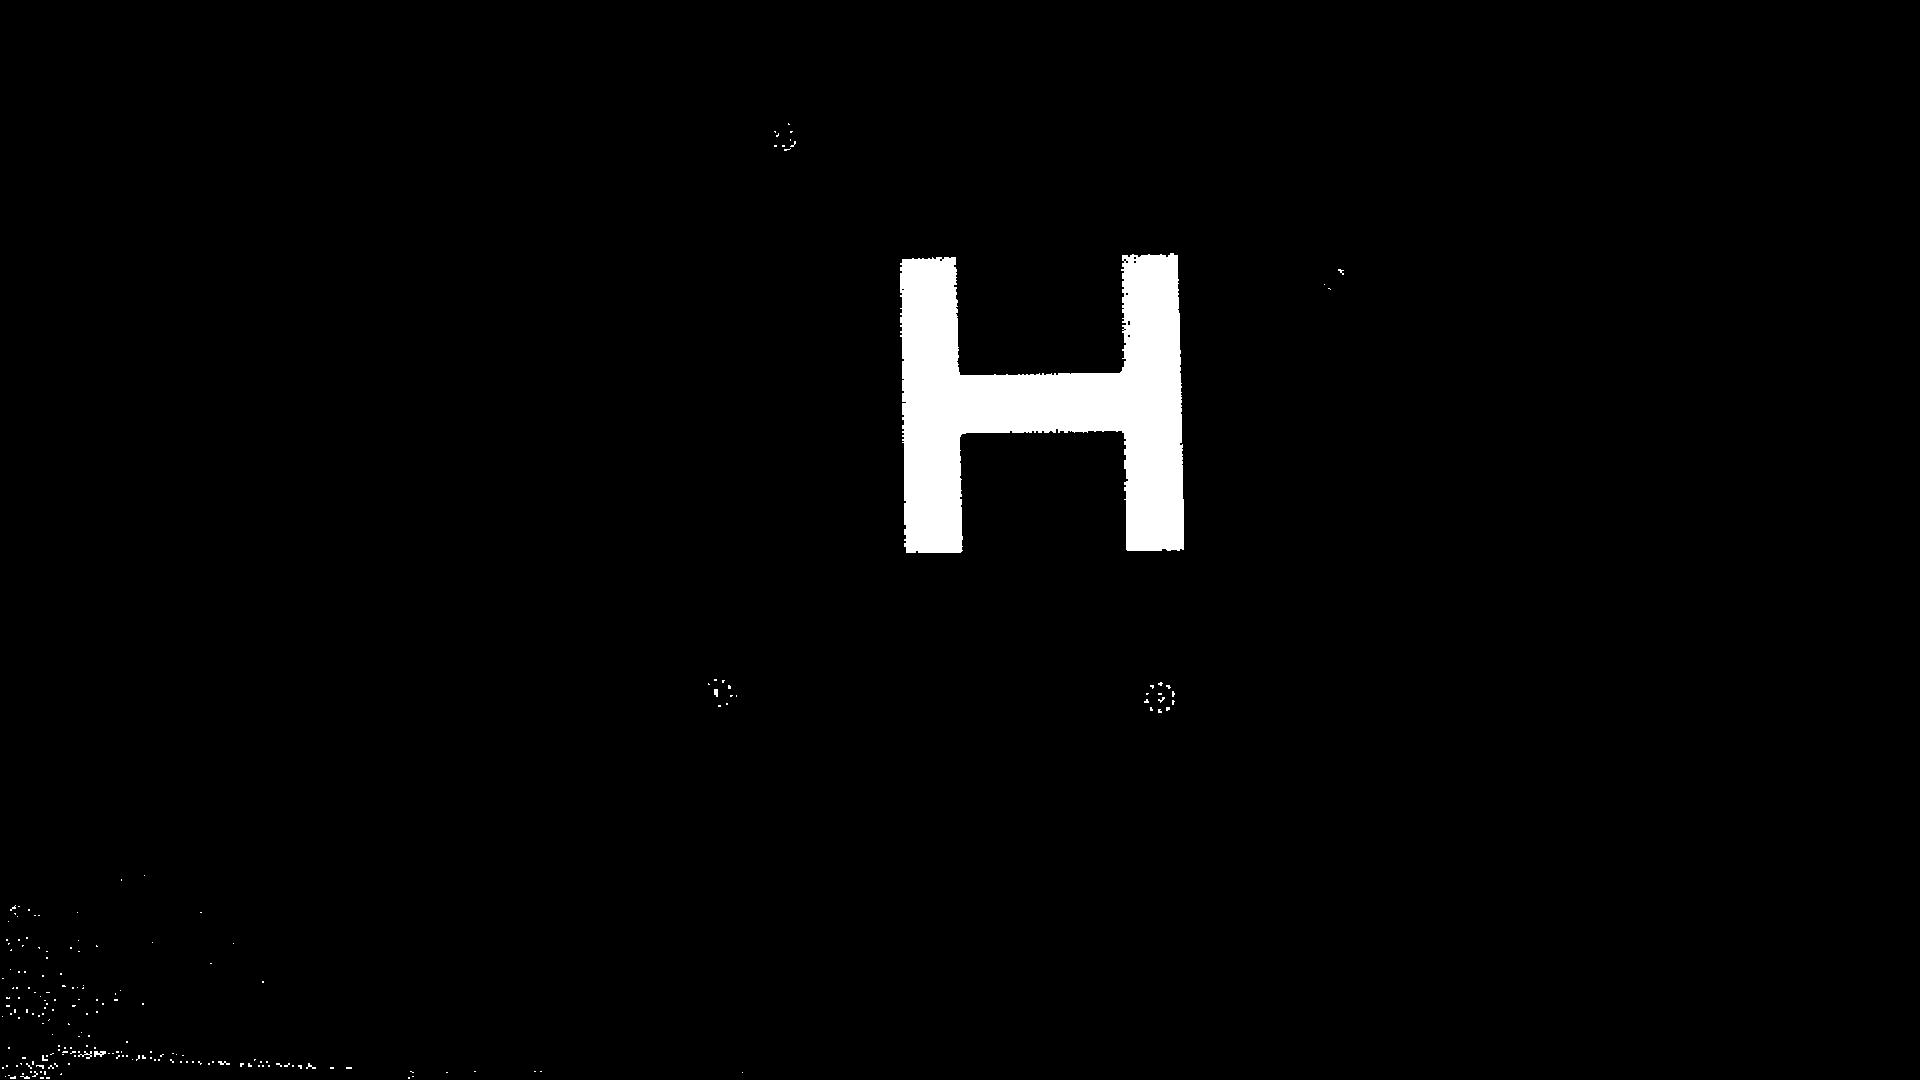
\includegraphics[width=\textwidth]{bin.jpg}
		\caption{Rezultat binaryzacji.}
		\label{fig:bin_1}
	\end{subfigure}
	\begin{subfigure}{0.7\textwidth}
		\centering
		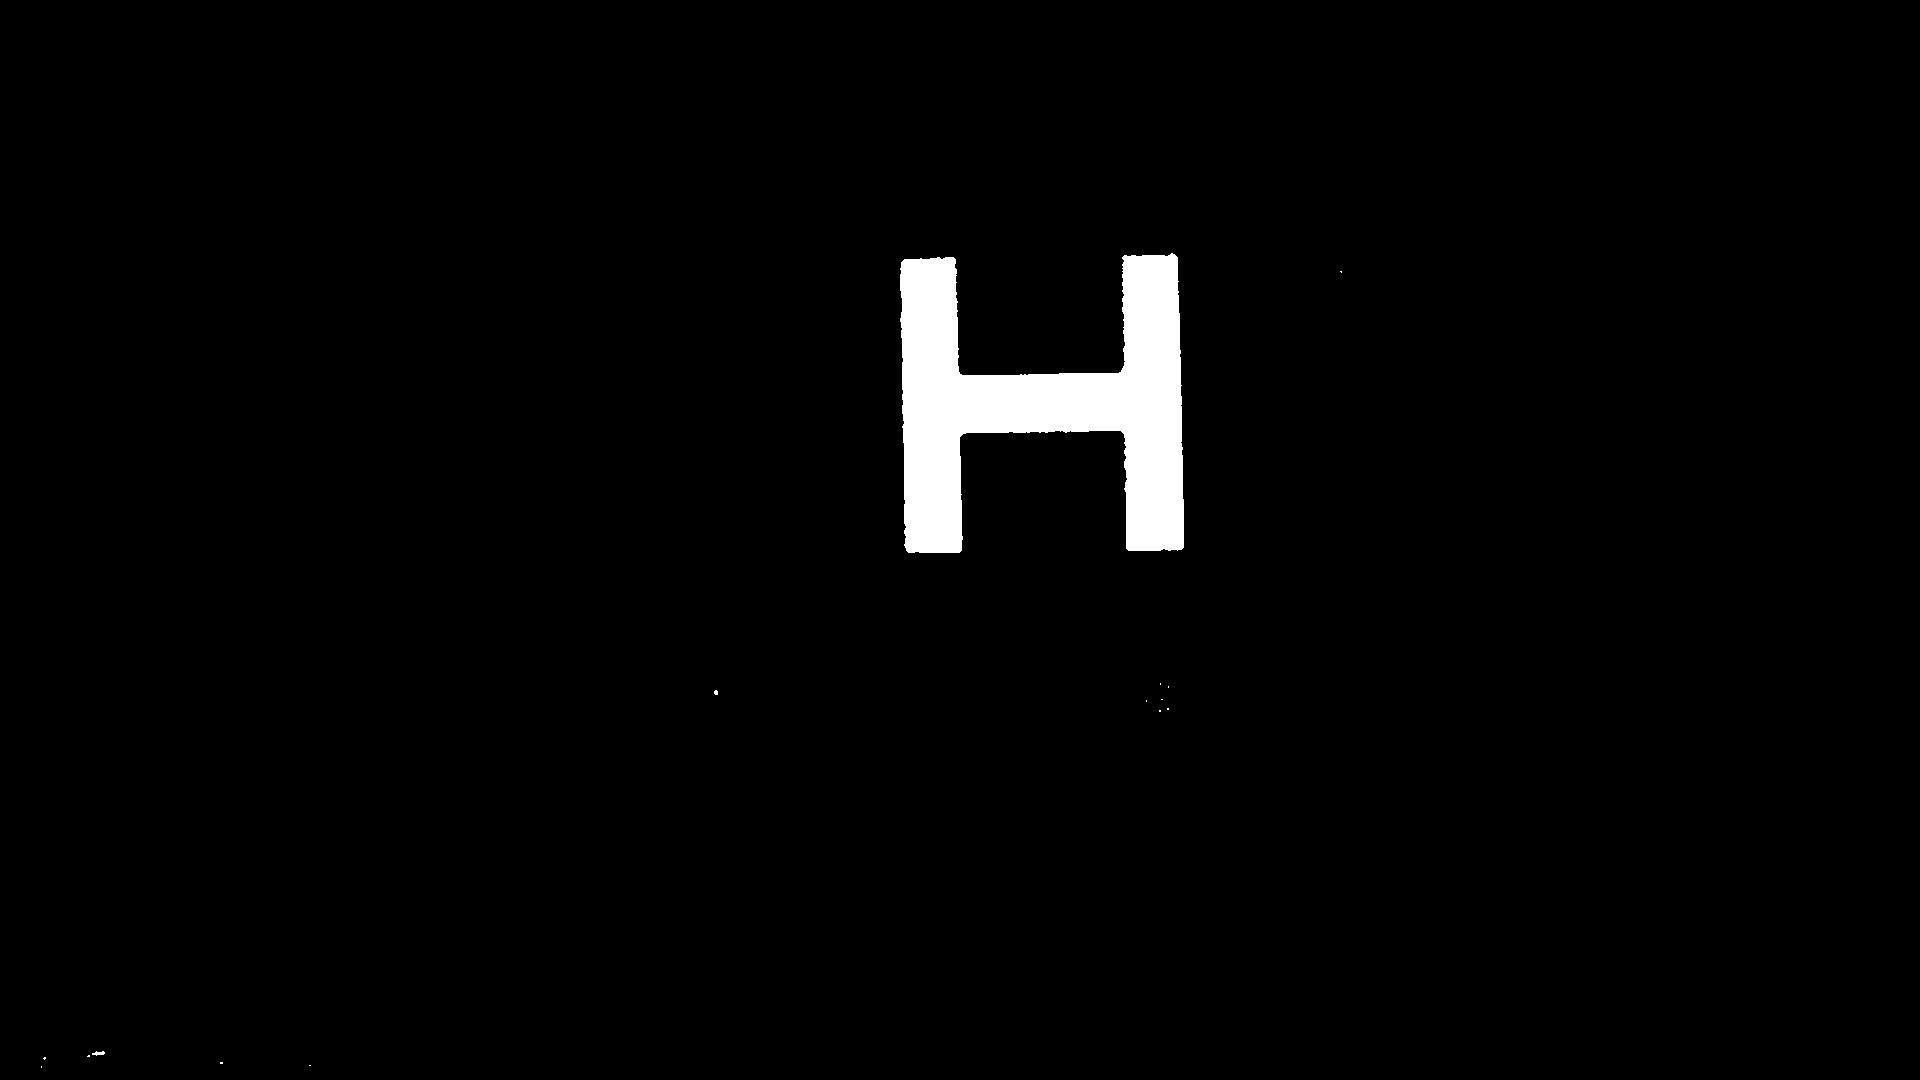
\includegraphics[width=\textwidth]{median.jpg}
		\caption{Obraz po medianie}
		\label{fig:median_1}
	\end{subfigure}\\
	\begin{subfigure}{0.7\textwidth}
		\centering
		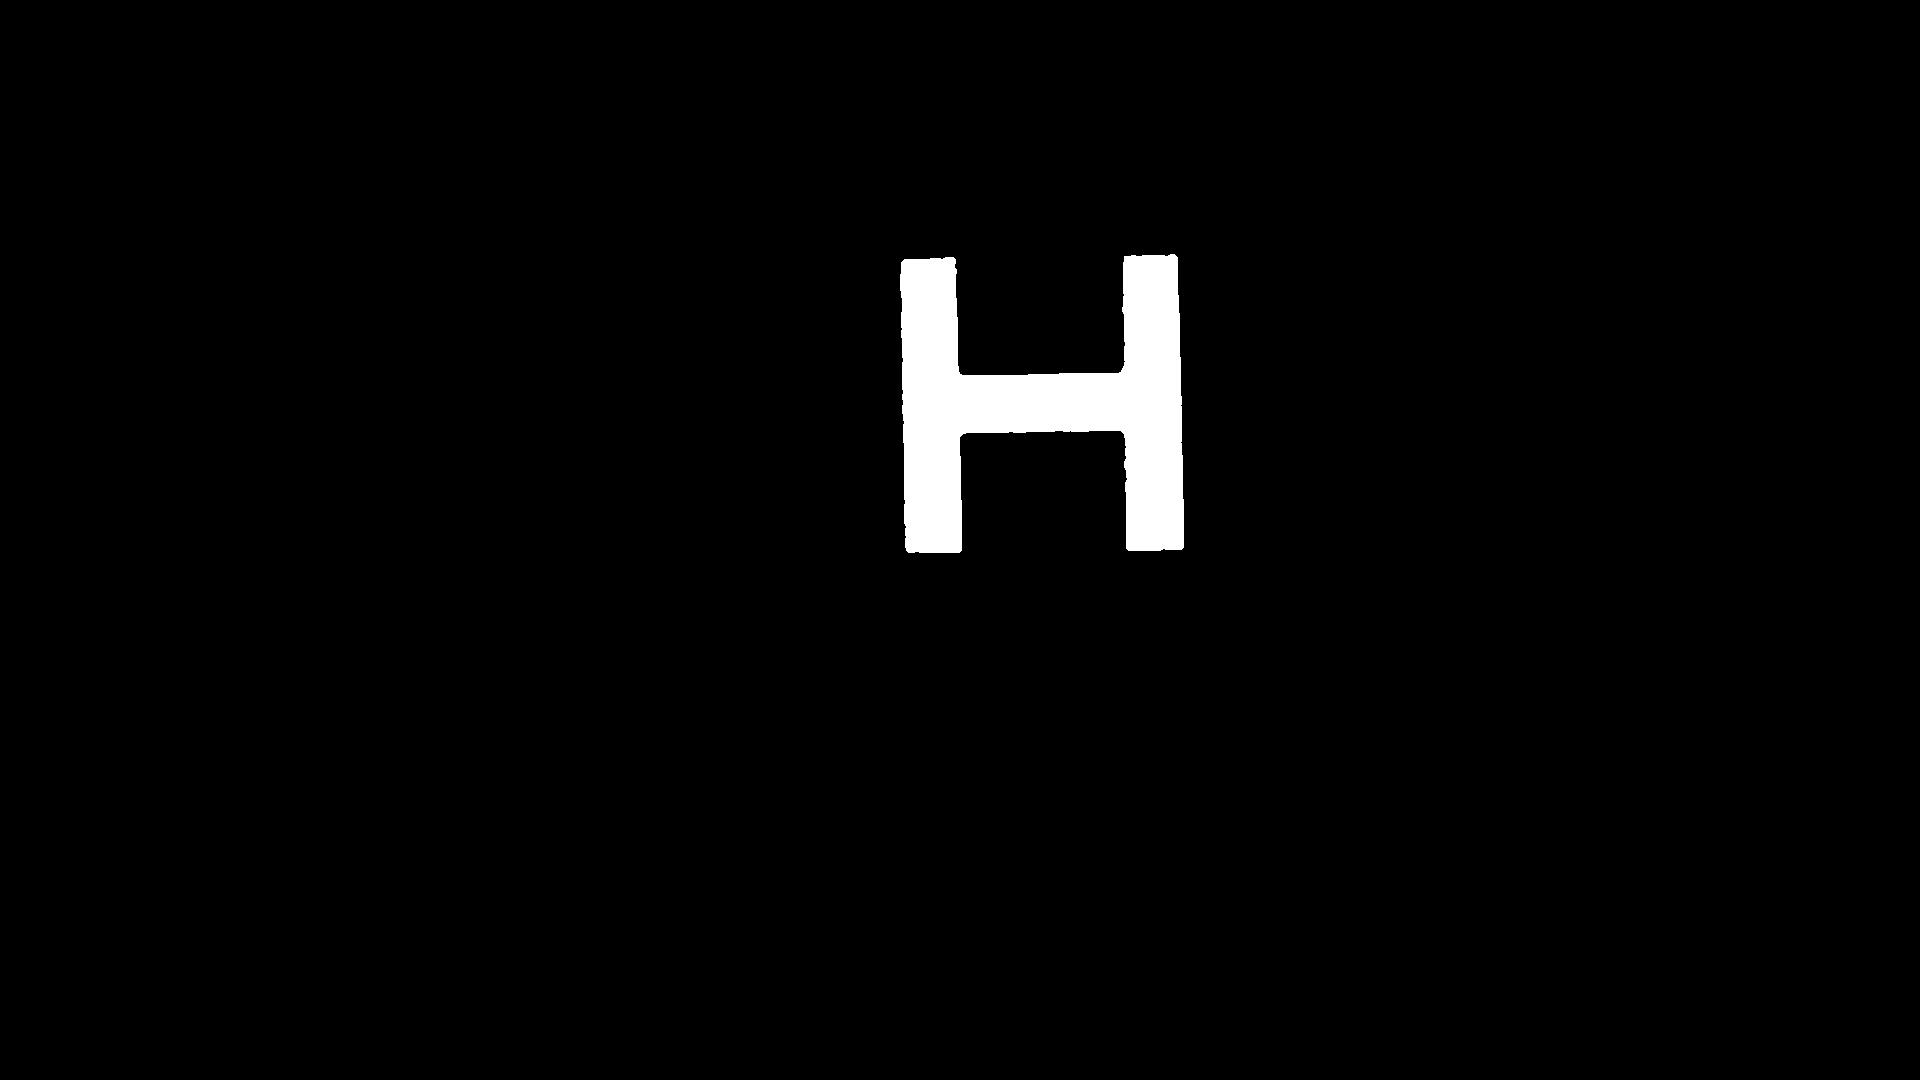
\includegraphics[width=\textwidth]{opened.jpg}
		\caption{Wynik otwarcia}
		\label{fig:opened_1}
	\end{subfigure}
	\caption{Przykładowe rezultaty binaryzacji, mediany i~otwarcia}
	\label{fig:operacje}
\end{figure}

%TODO2 Przydałby się obraz wejściowy. I nie ma potrzeby dawać tego takiego dużego. 4 obrazy w układzie 2x2 wystarczą.


\section{Wybór znacznika} 
\label{sec:wybor_znacznika}

Autonomiczne lądowanie drona w~oparciu o~system wizyjny wymaga wyposażenia lądowiska w~marker. 
Jego wygląd musi umożliwiać łatwą detekcję miejsca lądowania. 
Z~powodu wykonywania operacji na~zewnątrz, znacznik powinien również ułatwiać znalezienie go~w~zmiennych warunkach (zachmurzenie, cień).

\subsection{Kształt}
\label{subsec:ksztalt} 
Detekcja kształtów może być realizowana na~różne sposoby. 
Najprostszym jest progowanie współczynników kształtu, do~bardziej zaawansowanych należy wyspecjalizowana deskrypcja cech (SIFT, SURF, HOG) i~użycie klasyfikatorów (kNN, SVM, sieci neuronowe). %TODO2 skróty trzeba rozwinąć
W~implementowanej pierwszej wersji systemu zdecydowano się na~klasyfikację przy użyciu współczynnika kształtu.

Cechami obiektu łatwymi do~wyliczenia w~systemie potokowym są~pole figury i~najmniejszy prostokąt, w~którym figura się mieści (prostokąt otaczający). 
Postanowiono zatem wykorzystać współczynnik kształtu przedstawiony we~wzorze \ref{eq:wspolczynnik}.\\
\begin{equation} \label{eq:wspolczynnik}
W=\frac{P_p}{P_o}
\end{equation}
Gdzie:
\begin{eqwhere}[2cm]
	\item[$W$] współczynnik kształtu,
	\item[$P_p$] pole prostokąta otaczającego,
	\item[$P_o$] pole obiektu.
\end{eqwhere}
Aby~taki współczynnik umożliwiał detekcję należało dobrać odpowiedni kształt znacznika. 
Zdecydowano się na~krzyż, gdyż przy każdej jego orientacji pole prostokąta jest znacznie większe od~pola obiektu.

\subsection{Kolor}
\label{subsec:kolor}

Kolor znacznika powinien umożliwiać jego łatwą segmentację. 
Z~tego powodu pożądane jest silne skontrastowanie figury i~tła. 
Najbardziej naturalnym rozwiązaniem jest rozważenie kontrastu w~przestrzeni barw RGB, gdyż taki sygnał jest dostarczany przez kamerę.

\begin{figure}[h]
	\centering
	\begin{subfigure}{0.4\textwidth}
		\centering
		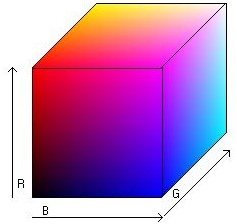
\includegraphics[width=0.5\textwidth]{szescian_rgb.jpg}
		\caption{Przedstawienie przestrzeni barw RGB w~postaci sześcianu \cite{obrazek_rgb}}
		\label{fig:szescian_rgb}
	\end{subfigure}%
	\begin{subfigure}{0.4\textwidth}
		\centering
		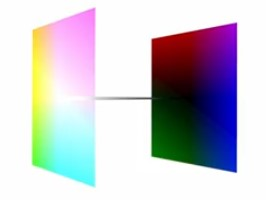
\includegraphics[width=0.5\textwidth]{szescian_ycbcr.jpg}
		\caption{Przekroje sześcianu przestrzeni YCbCr \cite{obrazek_ycbcr}}
		\label{fig:szescian_ycbcr}
	\end{subfigure}%
	\caption{Modele przestrzeni RGB i YCbCr}
	\label{fig:modele_przestrzeni}
\end{figure}

W~przestrzeni RGB każdy piksel opisywany jest przez trzy składowe: czerwoną, zieloną i~niebieską. 
Możliwe jest przedstawienie tego systemu w~formie sześcianu (rys. \ref{fig:szescian_rgb}). 
Można wyznaczyć przekątną łączącą punkty, dla których wszystkie współrzędne są~identyczne. 
Rozciąga się ona od~koloru czarnego w~początku układu współrzędnych, do~białego dla~maksymalnych wartości składowych, przechodząc przez różne stopnie szarości. 
Wykorzystanie dużej odległości między kolorami i~użycie czarno-białego znacznika wydaje się zatem najprostszym pomysłem.

W~pierwszym kroku do testów przygotowano czarny znacznik na~białym tle. 
Kamerą PCAM 5C wykonano trzy zdjęcia przy różnym poziomie oświetlenia (Rys. \ref{fig:osw1}, \ref{fig:osw2}, \ref{fig:osw3}). %TODO2 tu odnośnik do dalszej części pracy
Po~przejściu na~obraz w~skali szarości, posługując się narzędziem \textit{roipoly} w~programie Matlab, obliczono histogramy obszaru znacznika (rys. \ref{fig:bw_hist1}, \ref{fig:bw_hist2}, \ref{fig:bw_hist3}).\\
\begin{figure}
	\centering
	\begin{subfigure}{0.4\textwidth}
		\centering
		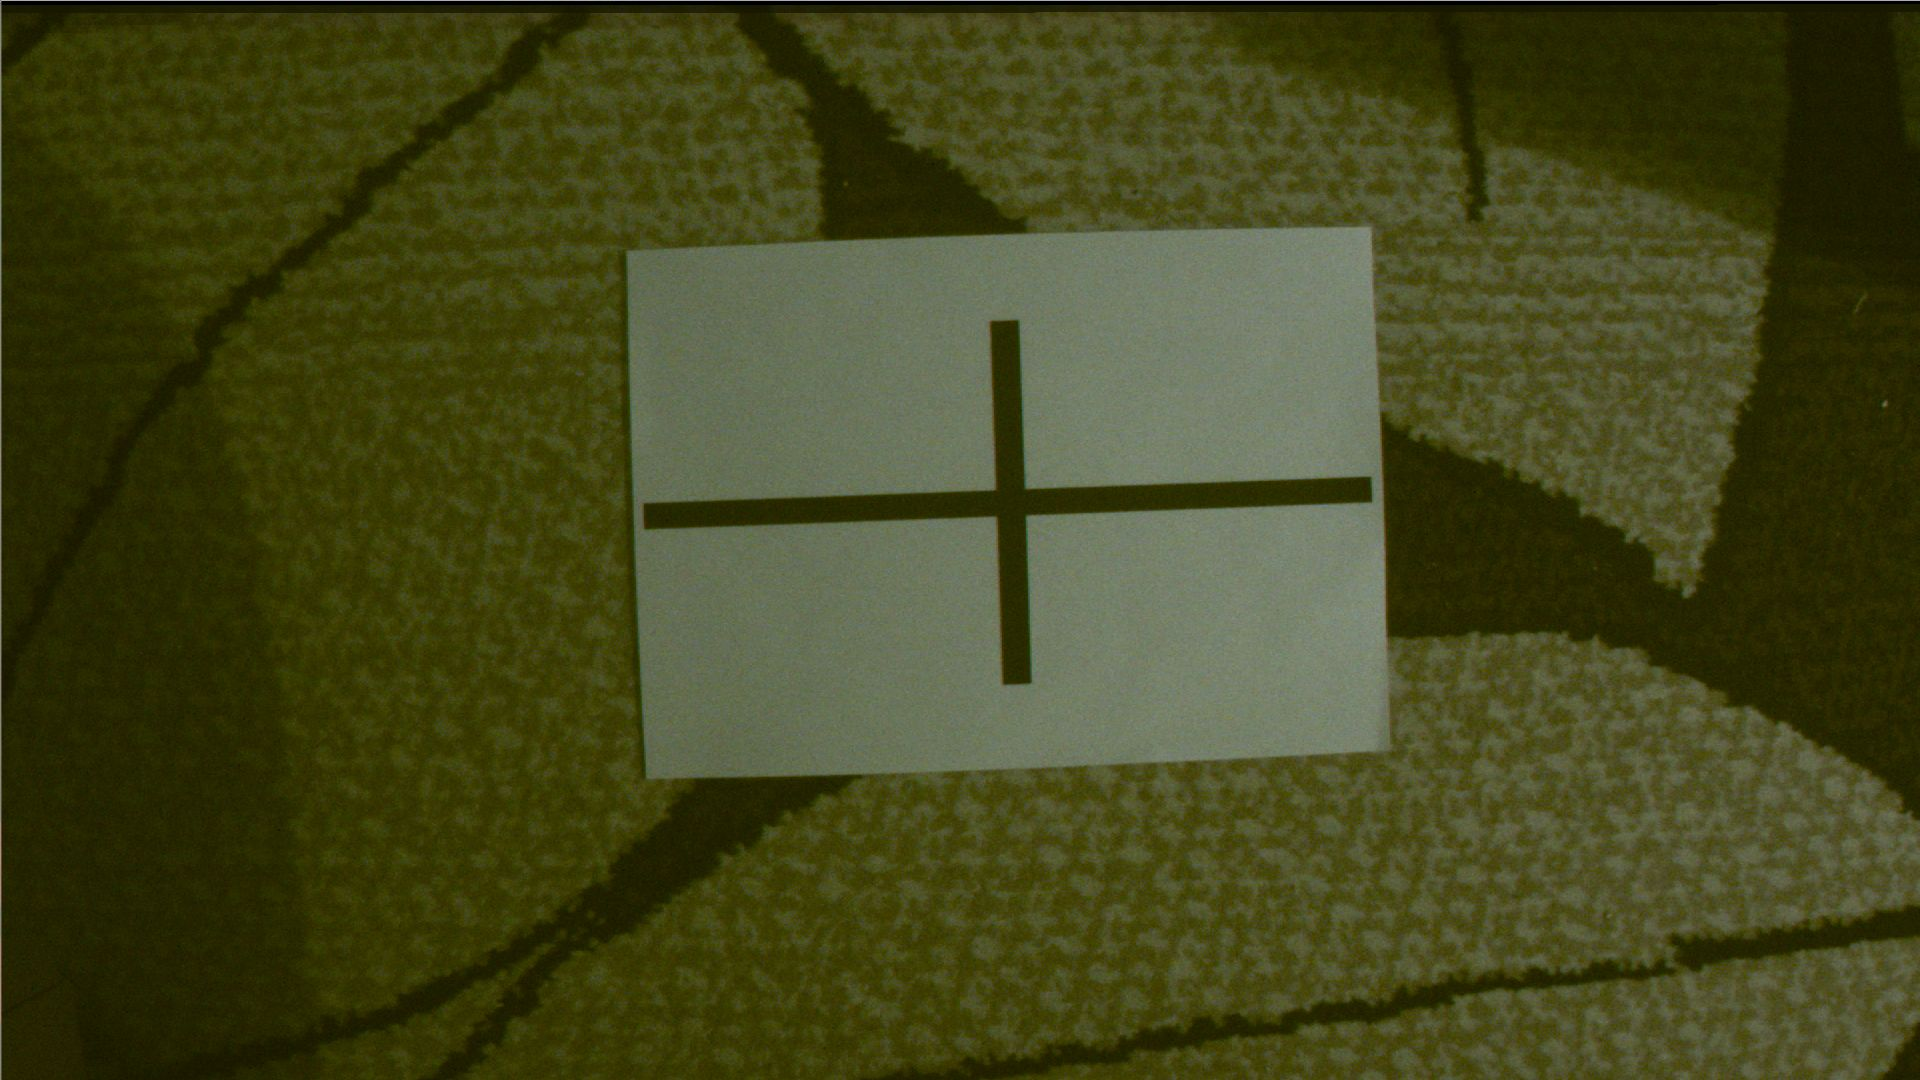
\includegraphics[width=0.98\textwidth]{rgb_ciemny.jpg}
		\caption{}
		\label{fig:osw1}
	\end{subfigure}%
	\begin{subfigure}{0.55\textwidth}
		\centering
		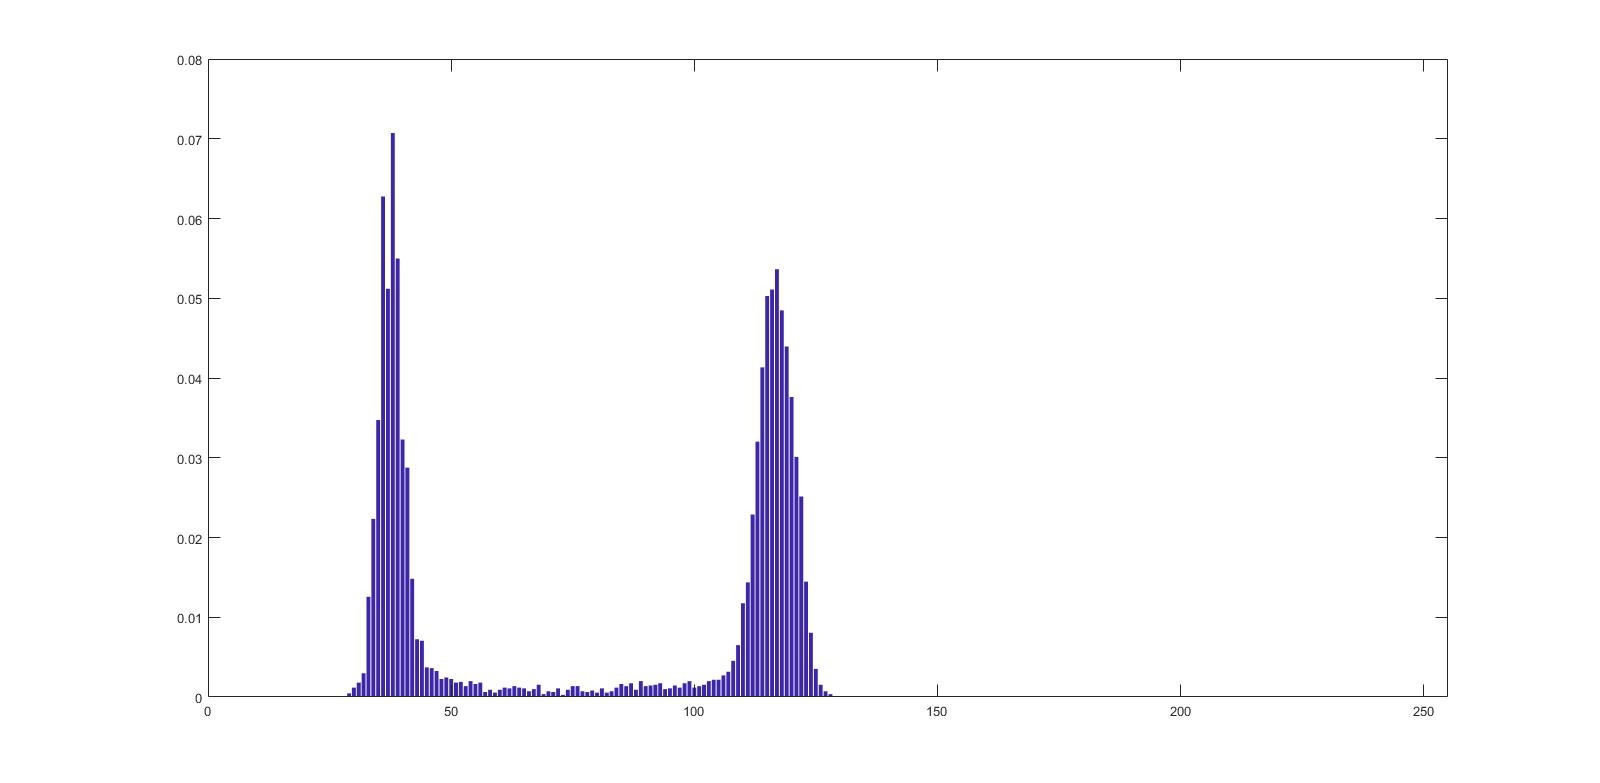
\includegraphics[width=0.98\textwidth]{bw_hist1.jpg}
		\caption{}
		\label{fig:bw_hist1}
	\end{subfigure}\\
	\begin{subfigure}{0.4\textwidth}
		\centering
		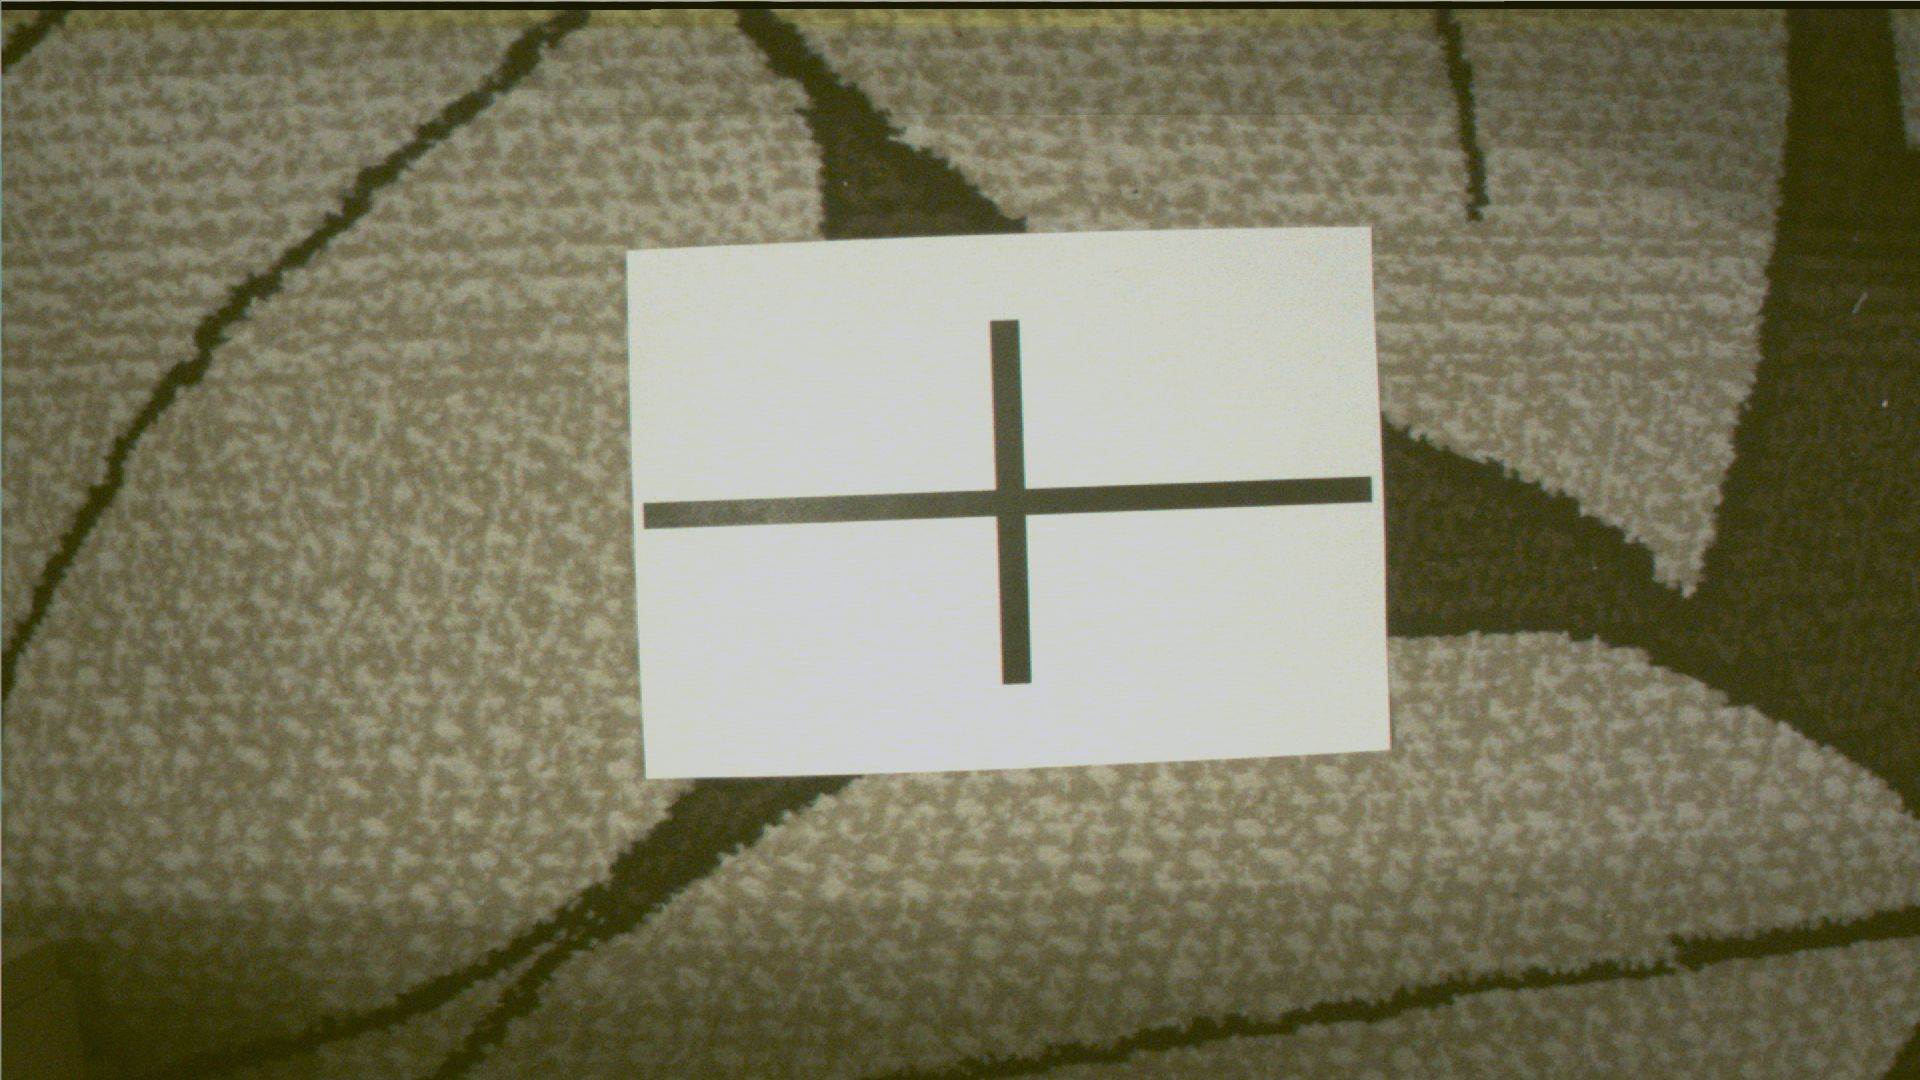
\includegraphics[width=0.98\textwidth]{rgb_sredni.jpg}
		\caption{}
		\label{fig:osw2}
	\end{subfigure}
	\begin{subfigure}{0.55\textwidth}
		\centering
		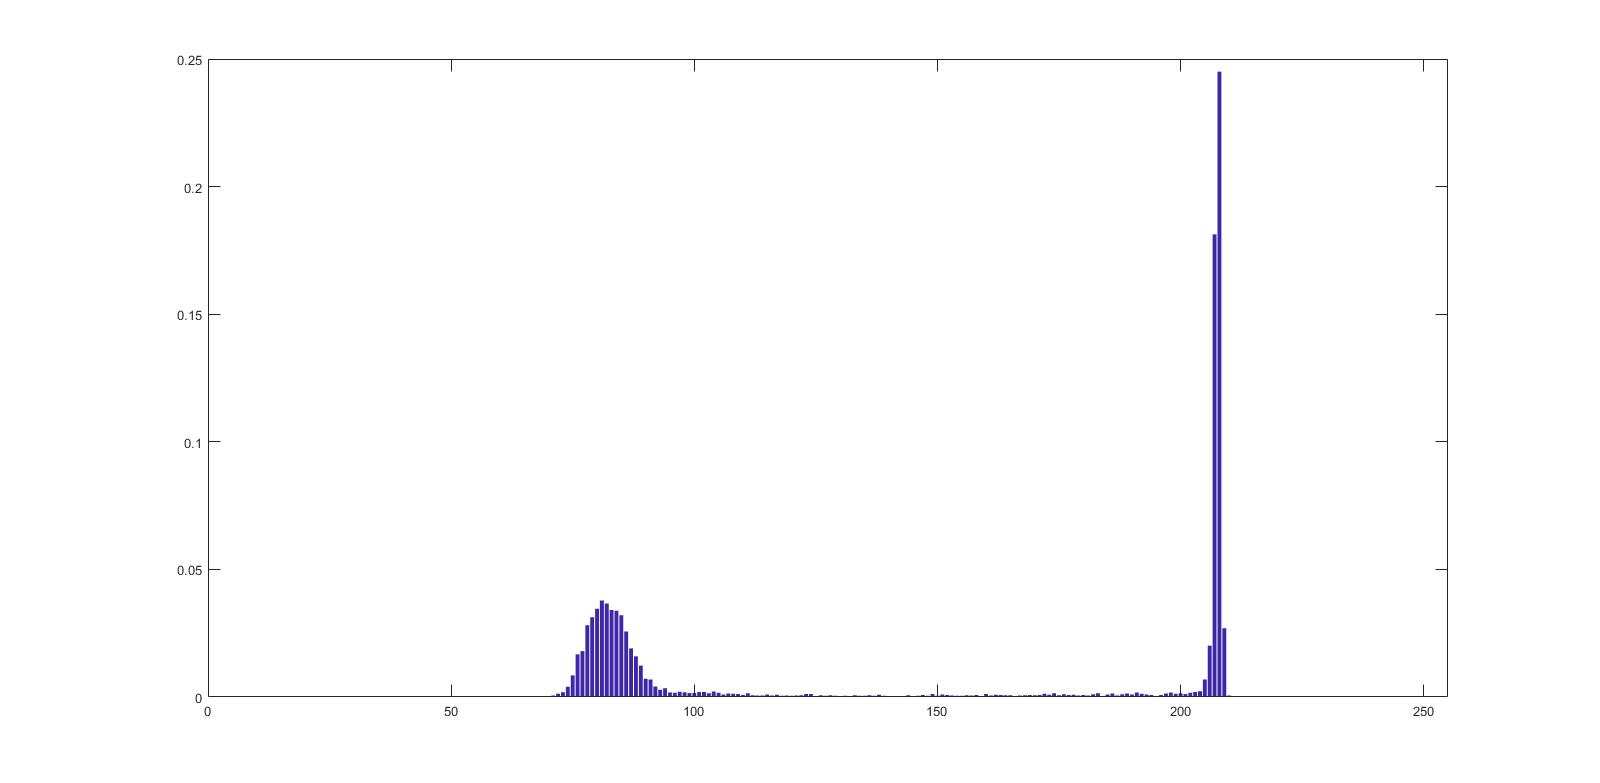
\includegraphics[width=0.98\textwidth]{bw_hist2.jpg}
		\caption{}
		\label{fig:bw_hist2}
	\end{subfigure}\\
	\begin{subfigure}{0.4\textwidth}
		\centering
		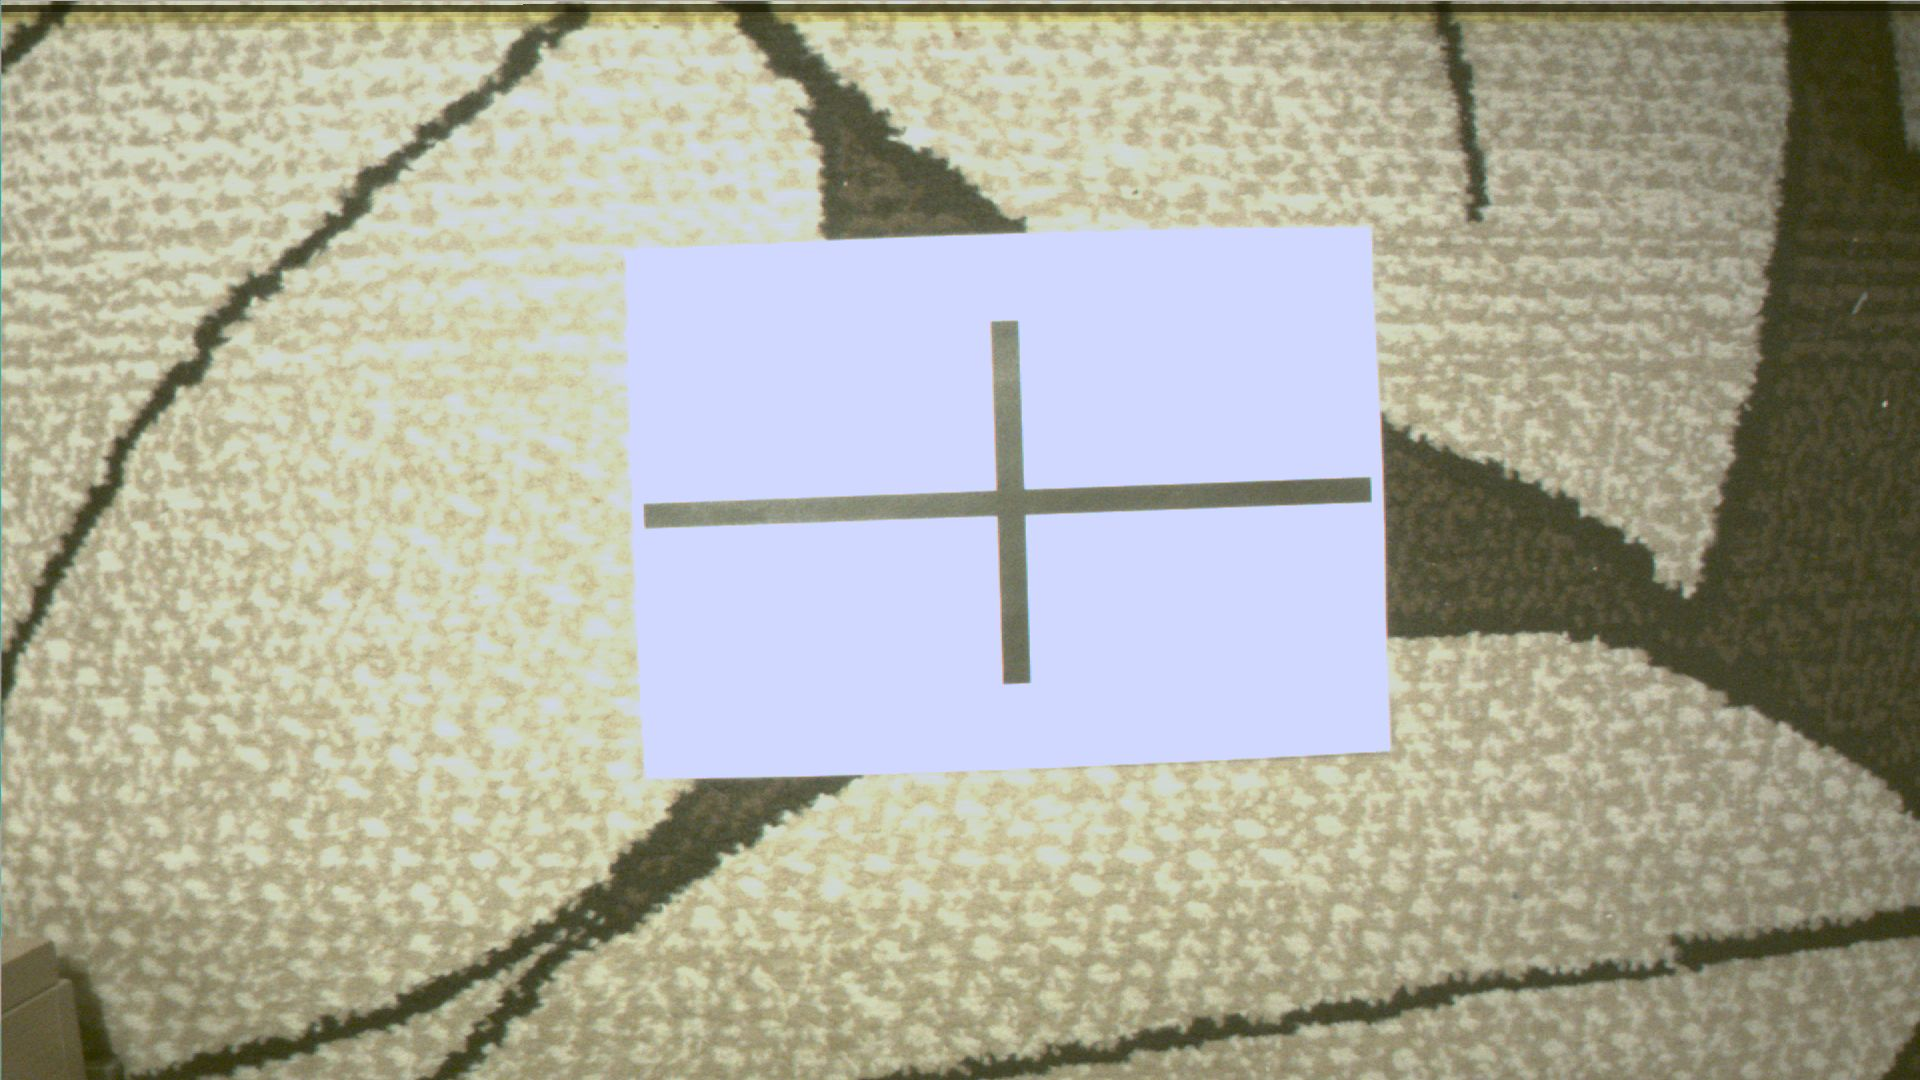
\includegraphics[width=0.98\textwidth]{rgb_jasny.jpg}
		\caption{}
		\label{fig:osw3}
	\end{subfigure}
	\begin{subfigure}{0.55\textwidth}
		\centering
		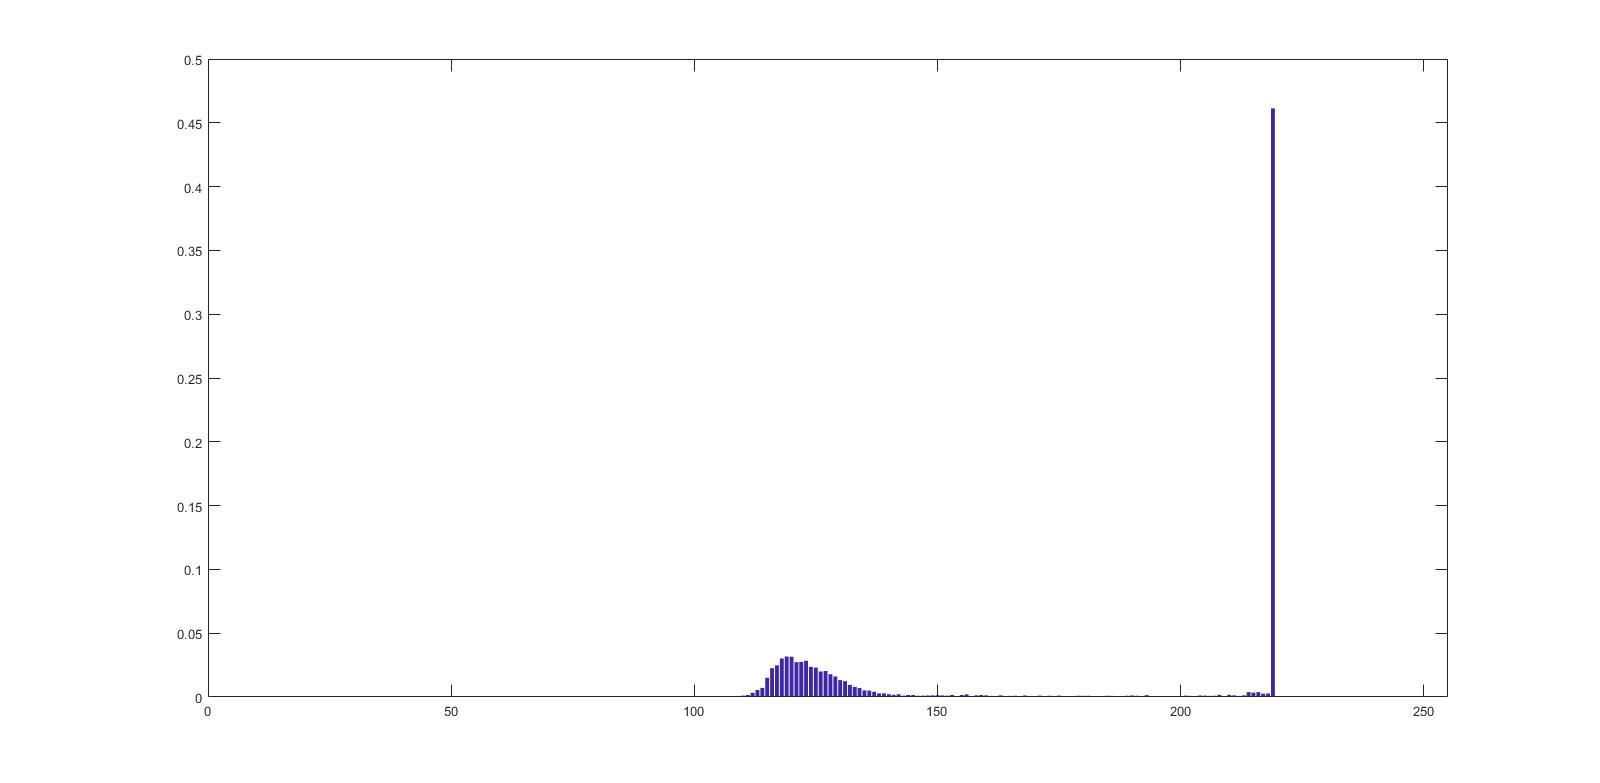
\includegraphics[width=0.98\textwidth]{bw_hist3.jpg}
		\caption{}
		\label{fig:bw_hist3}
	\end{subfigure}
	\caption{Zdjęcia pierwszej wersji znacznika wraz z~histogramami obszaru znacznika}
	\label{fig:zdjecia_wejsciowe}
\end{figure}

Analiza histogramów wskazuje na~silne uzależnienie wartości koloru od~oświetlenia.  %TODO2 raczej położenia maksimów odpowiadających tłu i znacznikowi.
Dla kolejnych obrazów, wartości progów binaryzacji mogłyby zawierać się w~zakresach: 50-100, 100-200, 150-210. Poziom białego tła dla obrazka najsłabiej oświetlonego jest mniejszy niż wartość czarnego koloru znacznika najlepiej oświetlonego. 
W~takiej sytuacji niemożliwy jest dobór stałego progu umożliwiającego skuteczną binaryzację.

Z~tego powodu zdecydowano się na~powtórzenie eksperymentu w~przestrzeni YCbCr. 
Tak jak opisano w~rozdziale \ref{sec:implementacja_modelu_programowego}, piksel w~tej przestrzeni opisuje współrzędna luminancji i~dwie składowe chrominacji. 
Podobnie jak w~przypadku RGB, przestrzeń YCbCr również da~się przedstawić w~postaci sześcianu. 
Tym razem skala szarości przebiega przez środek płaszczyzn Cb-Cr i~za zmianę poziomu szarości odpowiada współrzędna luminancji (rys. \ref{fig:szescian_ycbcr}). 
Dla~każdej wartości piksela informacja o~jasności oddzielona jest od~barwy.

Kolor znacznika określono jako czerwony, natomiast tło niebieskie, gdyż te~barwy znajdują się na~przeciwnych stronach płaszczyzny Cr-Cb. 
Zdjęcia wykonano przy takich samych poziomach oświetlenia jak poprzednio. 
Histogramy kolejnych obrazów przedstawiono na~rysunku \ref{fig:ycbcr_hist1}, \ref{fig:ycbcr_hist2}, \ref{fig:ycbcr_hist3}. 
\begin{figure}
	\centering
	\begin{subfigure}{\textwidth}
		\centering
		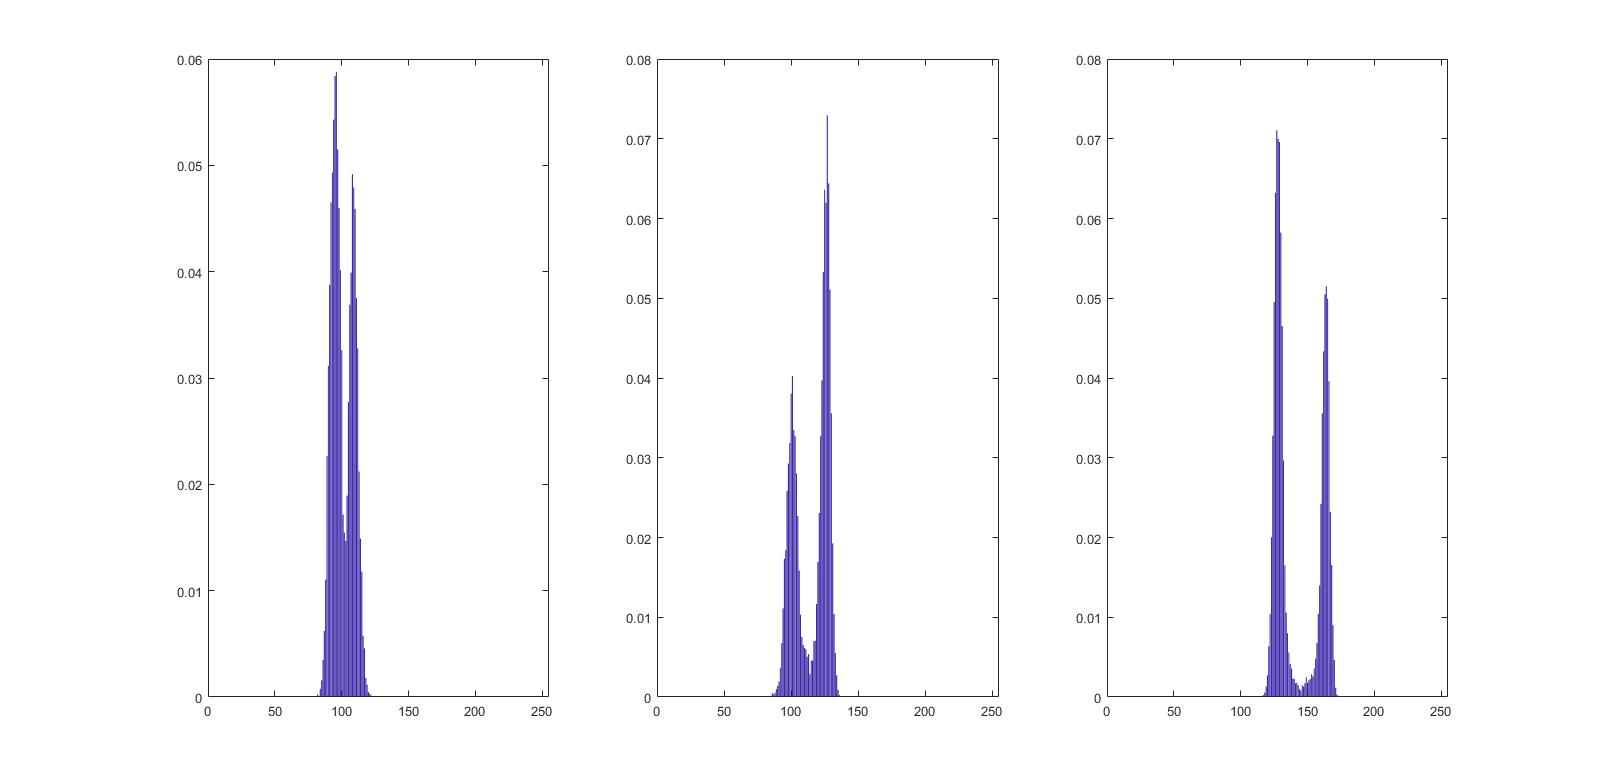
\includegraphics[width=0.9\textwidth]{ycbcr_hist1.jpg}
		\caption{}
		\label{fig:ycbcr_hist1}
	\end{subfigure}\\
	\begin{subfigure}{\textwidth}
		\centering
		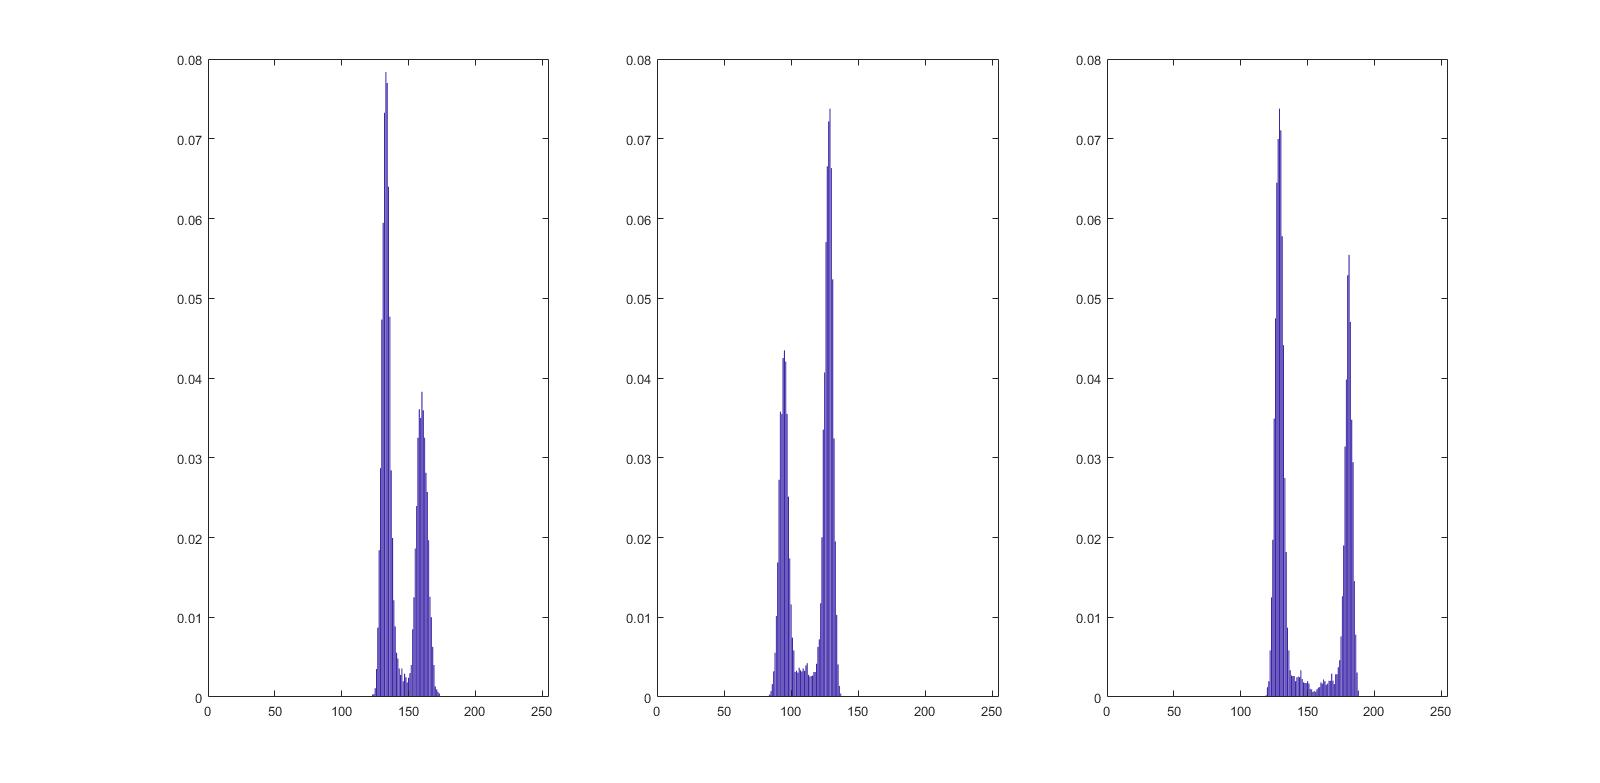
\includegraphics[width=0.9\textwidth]{ycbcr_hist2.jpg}
		\caption{}
		\label{fig:ycbcr_hist2}
	\end{subfigure}\\
	\begin{subfigure}{\textwidth}
		\centering
		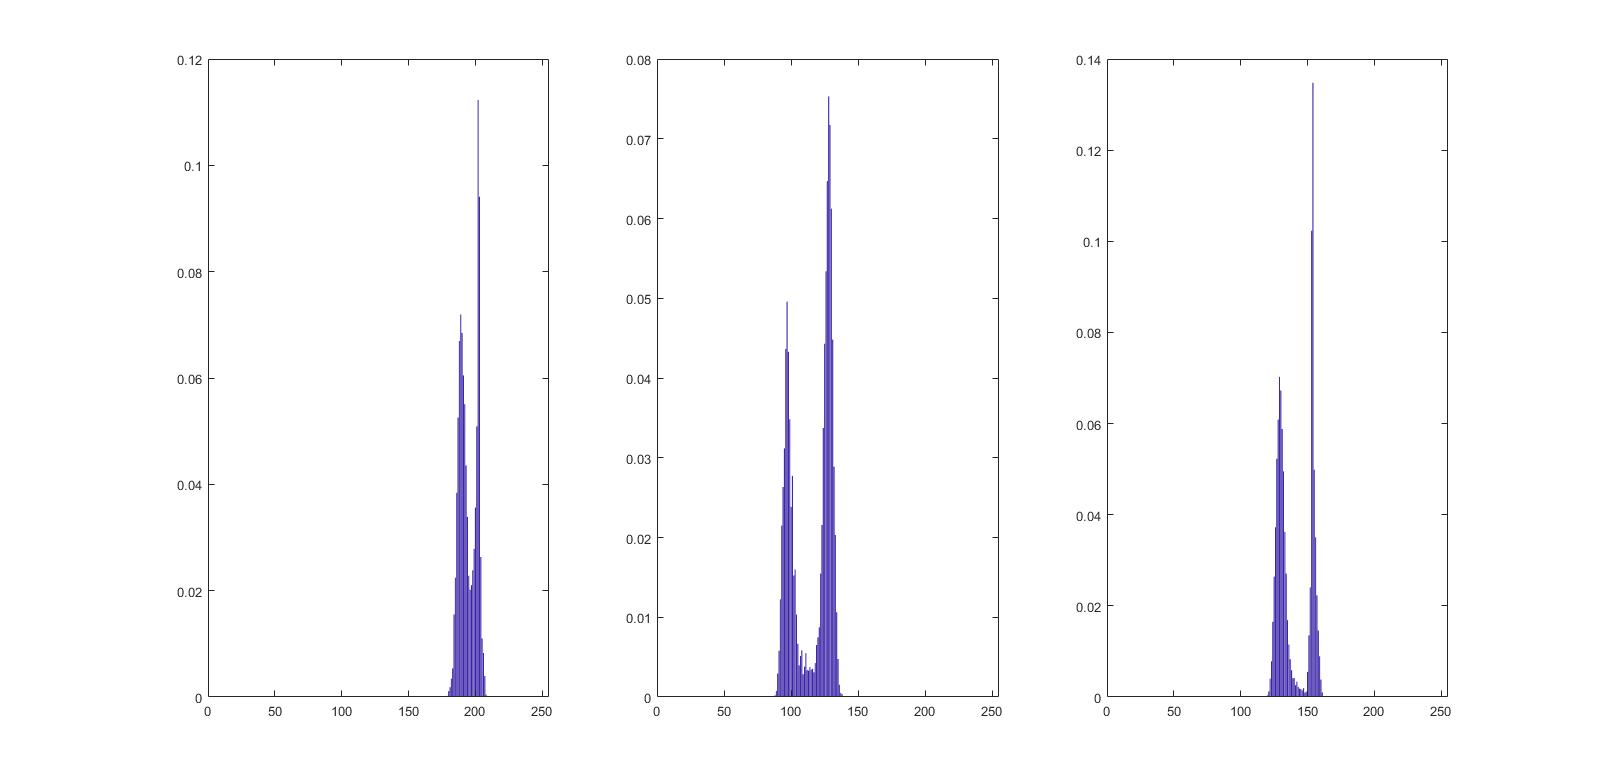
\includegraphics[width=0.9\textwidth]{ycbcr_hist3.jpg}
		\caption{}
		\label{fig:ycbcr_hist3}
	\end{subfigure}
	\caption{Histogramy obszarów znacznika w~przestrzeni YCbCr.}
	\label{fig:histogramy_ycbcr}
\end{figure}
%TODO2 Super by było jakby jednak na rysunku pojawiły się obrazy wejściowe.

Zgodnie z~oczekiwaniami, zmiana poziomu oświetlenia przełożyła~się na~zmianę wartości luminancji, natomiast składowe chrominancji nie zmieniały się znacząco. 
Każdy z~obrazów może być skutecznie zbinaryzowany przy użyciu stałych progów: górnego 120 dla składowej Cb i~dolnego 150 dla składowej Cr. 
Różnice pomiędzy wartościami składowych dla znacznika i~tła nie są jednak duże -- wynoszą około 30 poziomów. 
Ostatecznie zdecydowano się na~znacznik przedstawiony na~rys. \ref{fig:znacznik}.
\begin{figure}[h]
	\centering
	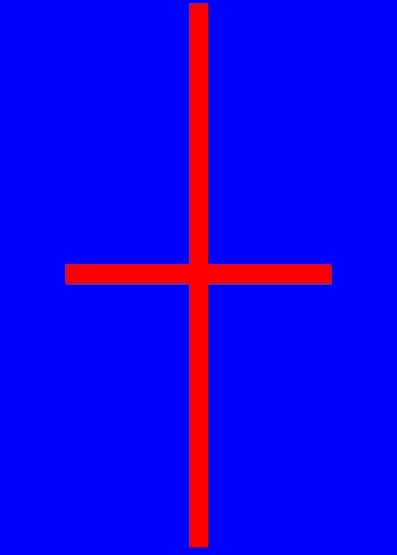
\includegraphics[width=0.3\textwidth]{znacznik.jpg}
	\caption{Wybrana postać znacznika}
	\label{fig:znacznik}
\end{figure}

%TODO2 Nic nigdzie nie pisze Pan o orientacji. Wiem, że nie ma detekcji, ale jakieś zdanie komentarza ?


\section{Analiza kąta widzenia kamery przy różnych ustawieniach rozdzielczości}
\label{sec:wyznaczenie_kata_widzenia_kamery_przy_roznych_ustawieniach}
W~celu zbadania kąta widzenia kamery stworzono moduł nakładający na~obraz prostopadłe linie przecinające się w~jego środku. %TODO2 to znowu odniesienie do tego rozdziału o SD
Następnie umieszczono kamerę na wysokości 49 cm i~skierowano ją w~dół. 
Odczytanie odległości od~środka obrazu do~jego krawędzi w~poziomie i~pionie pozwoliło na wyznaczenie kątów widzenia kamery. 
Skorzystano ze wzoru \eqref{eq:kat}.
\begin{equation}
\label{eq:kat}
\alpha=\arctan{\frac{l}{h}}
\end{equation}
gdzie:
\begin{eqwhere}[2cm]
	\item[$\alpha$] kąt widzenia kamery,
	\item[$h$] wysokość, na jakiej umieszczona jest kamera,
	\item[$l$] odległość środka obrazu od jego krawędzi.
\end{eqwhere}
Na podstawie obrazu przedstawionego na rysunku \ref{fig:1080p} obliczono kąty widzenia kamery w~pionie i~poziomie dla rozdzielczości 1920 x 1080. 
Dla rozdzielczości 1280 x 720 skorzystano z~obrazu pokazanego na rysunku \ref{fig:720p}. 
Korzystając ze wzoru \eqref{eq:kat} otrzymano przybliżone wyniki, przedstawione w tabeli \ref{tab:rozdzielczosc}.
\begin{table}[]
	\caption{Wartości kąta widzenia kamery w zależności od rozdzielczości}
	\label{tab:rozdzielczosc}
	\centering
	\begin{tabular}{|c|c|c|}
		\hline
		\begin{tabular}[c]{@{}c@{}}Rozdzielczość\end{tabular} &  Kąt widzenia kamery w pionie w stopniach  &  Kąt widzenia kamery w poziomie w stopniach  \\ \hline
		1920 x 1080                                                                          & 14 & 27 \\ \hline
		1280 x 720                                                                         & 19 & 38 \\ \hline
	\end{tabular}
\end{table}
\begin{figure}[h]
	\centering
	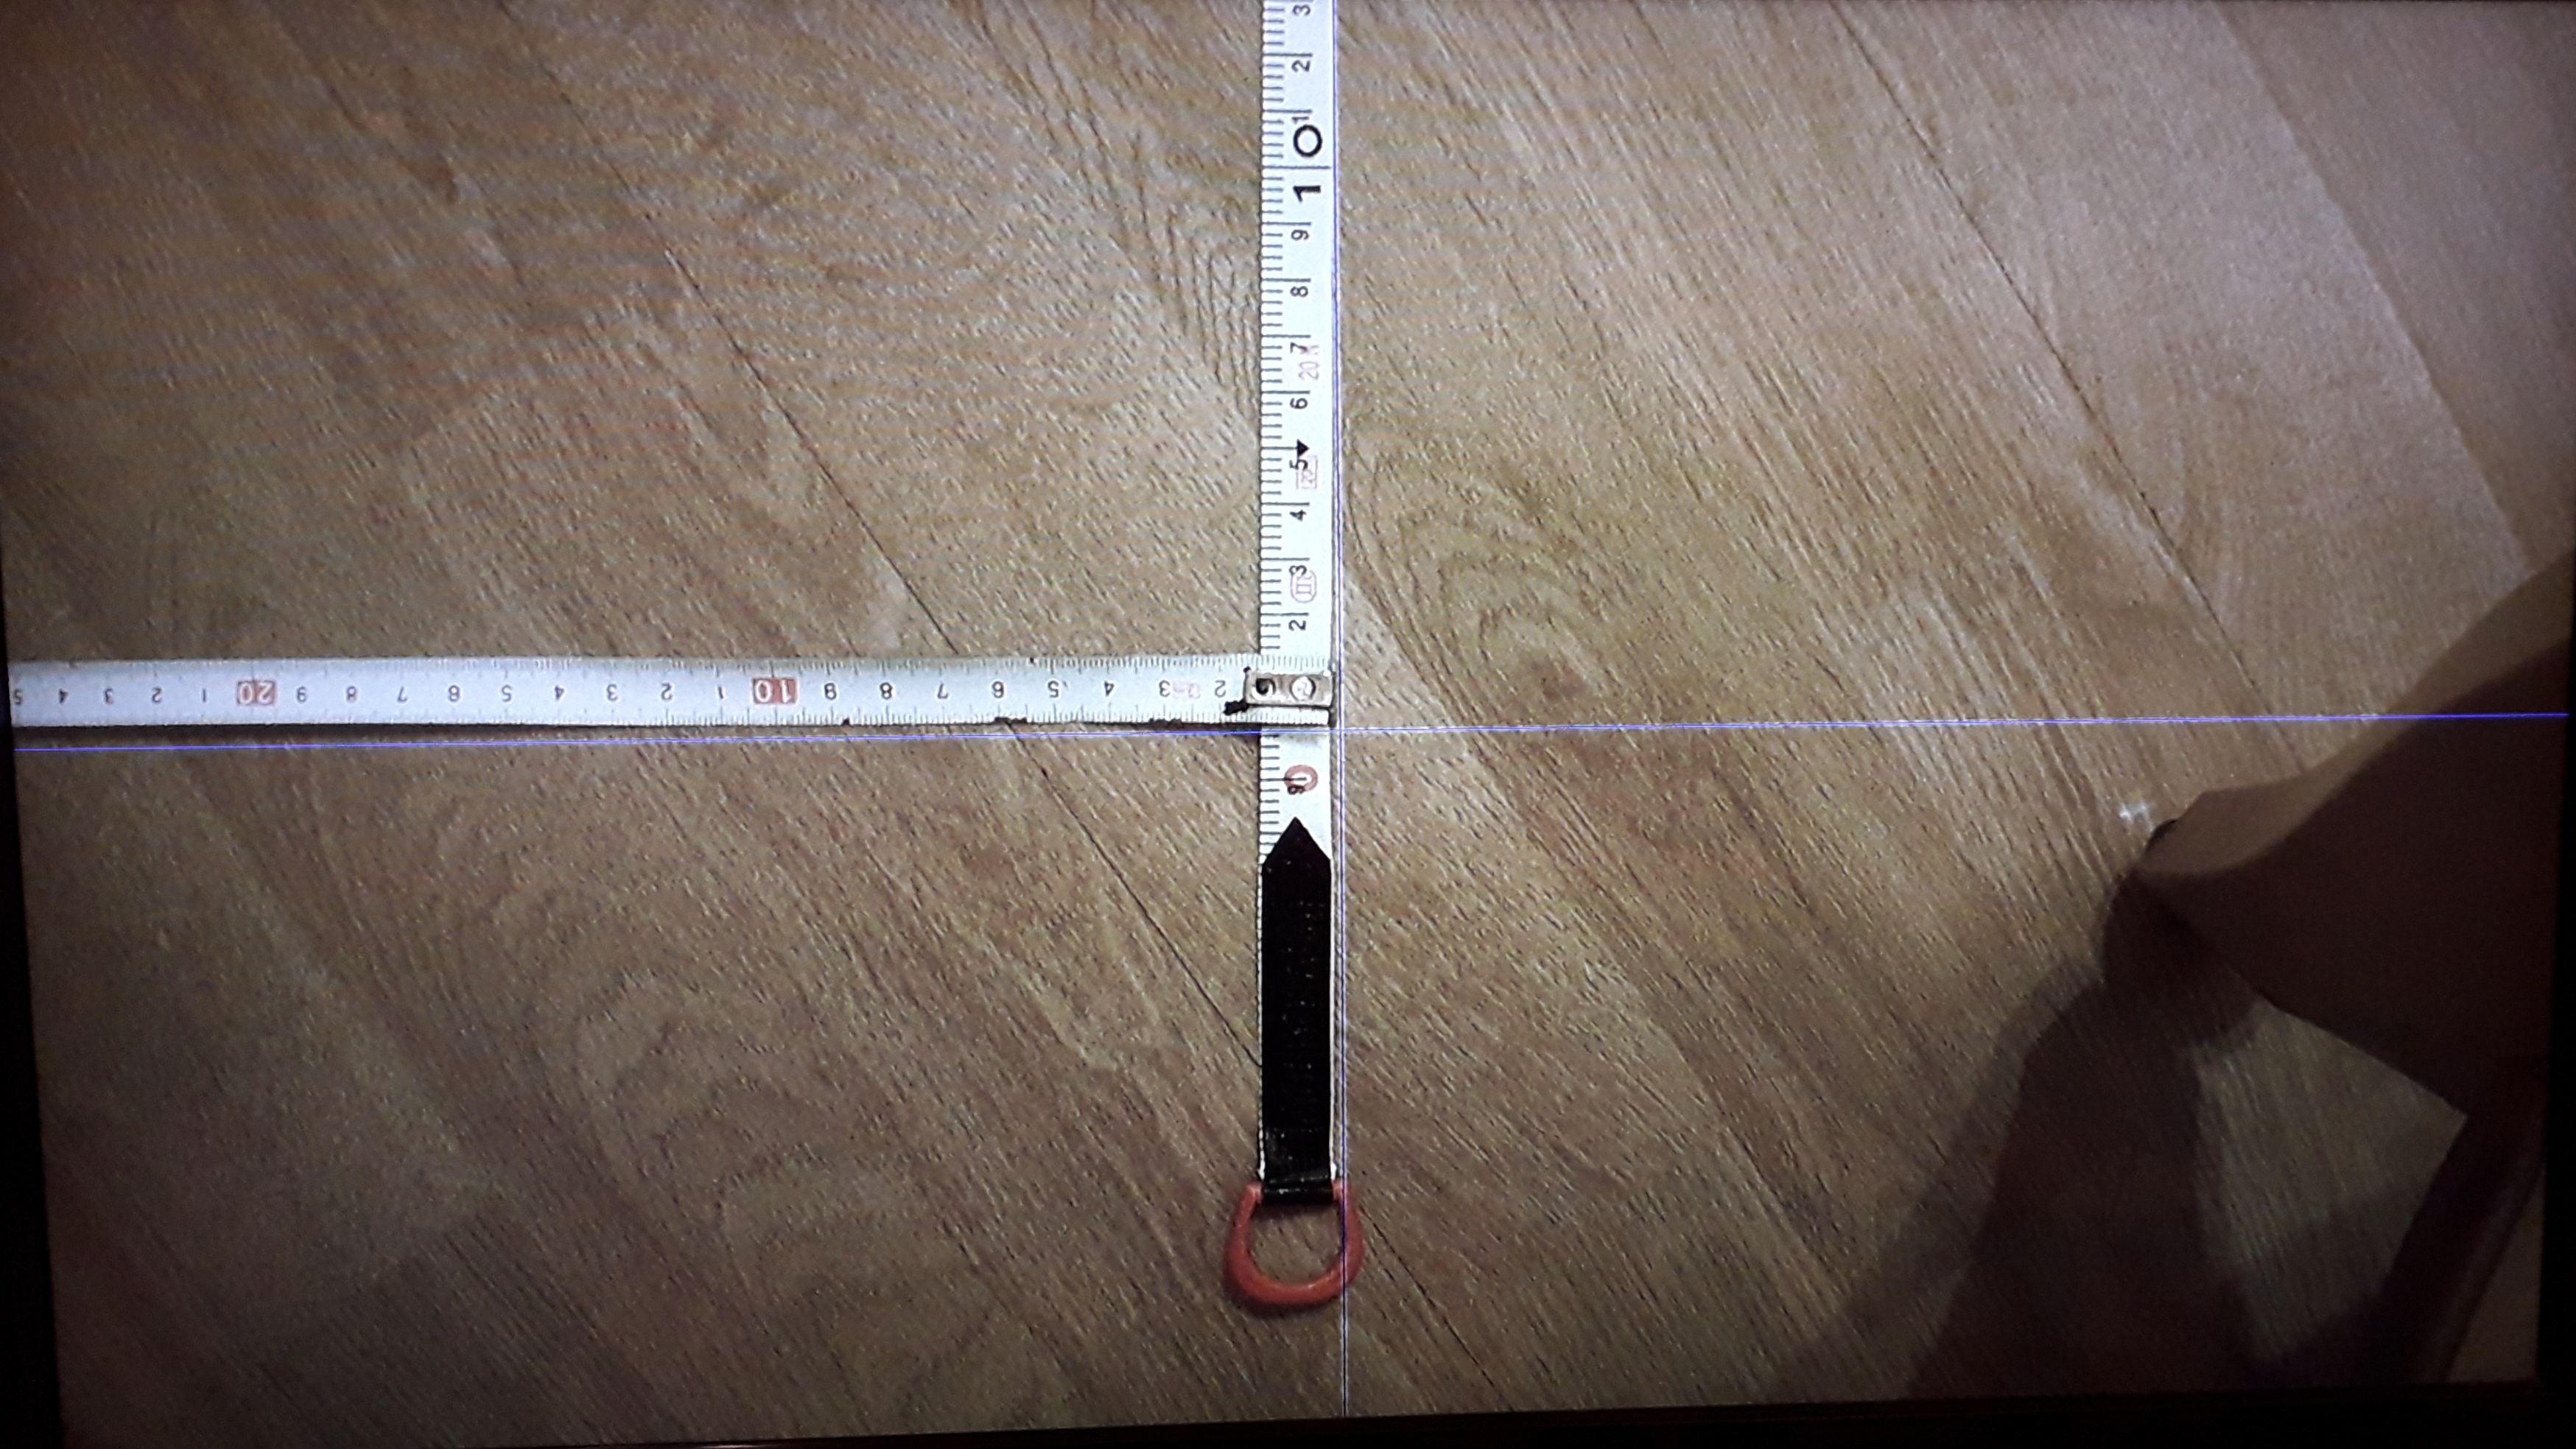
\includegraphics[width=\textwidth]{1080p.jpg}
	\caption{Obraz służący do wyznaczenia kąta widzenia kamery dla rozdzielczości 1920 x 1080.}
	\label{fig:1080p}
\end{figure}
\begin{figure}[h]
	\centering
	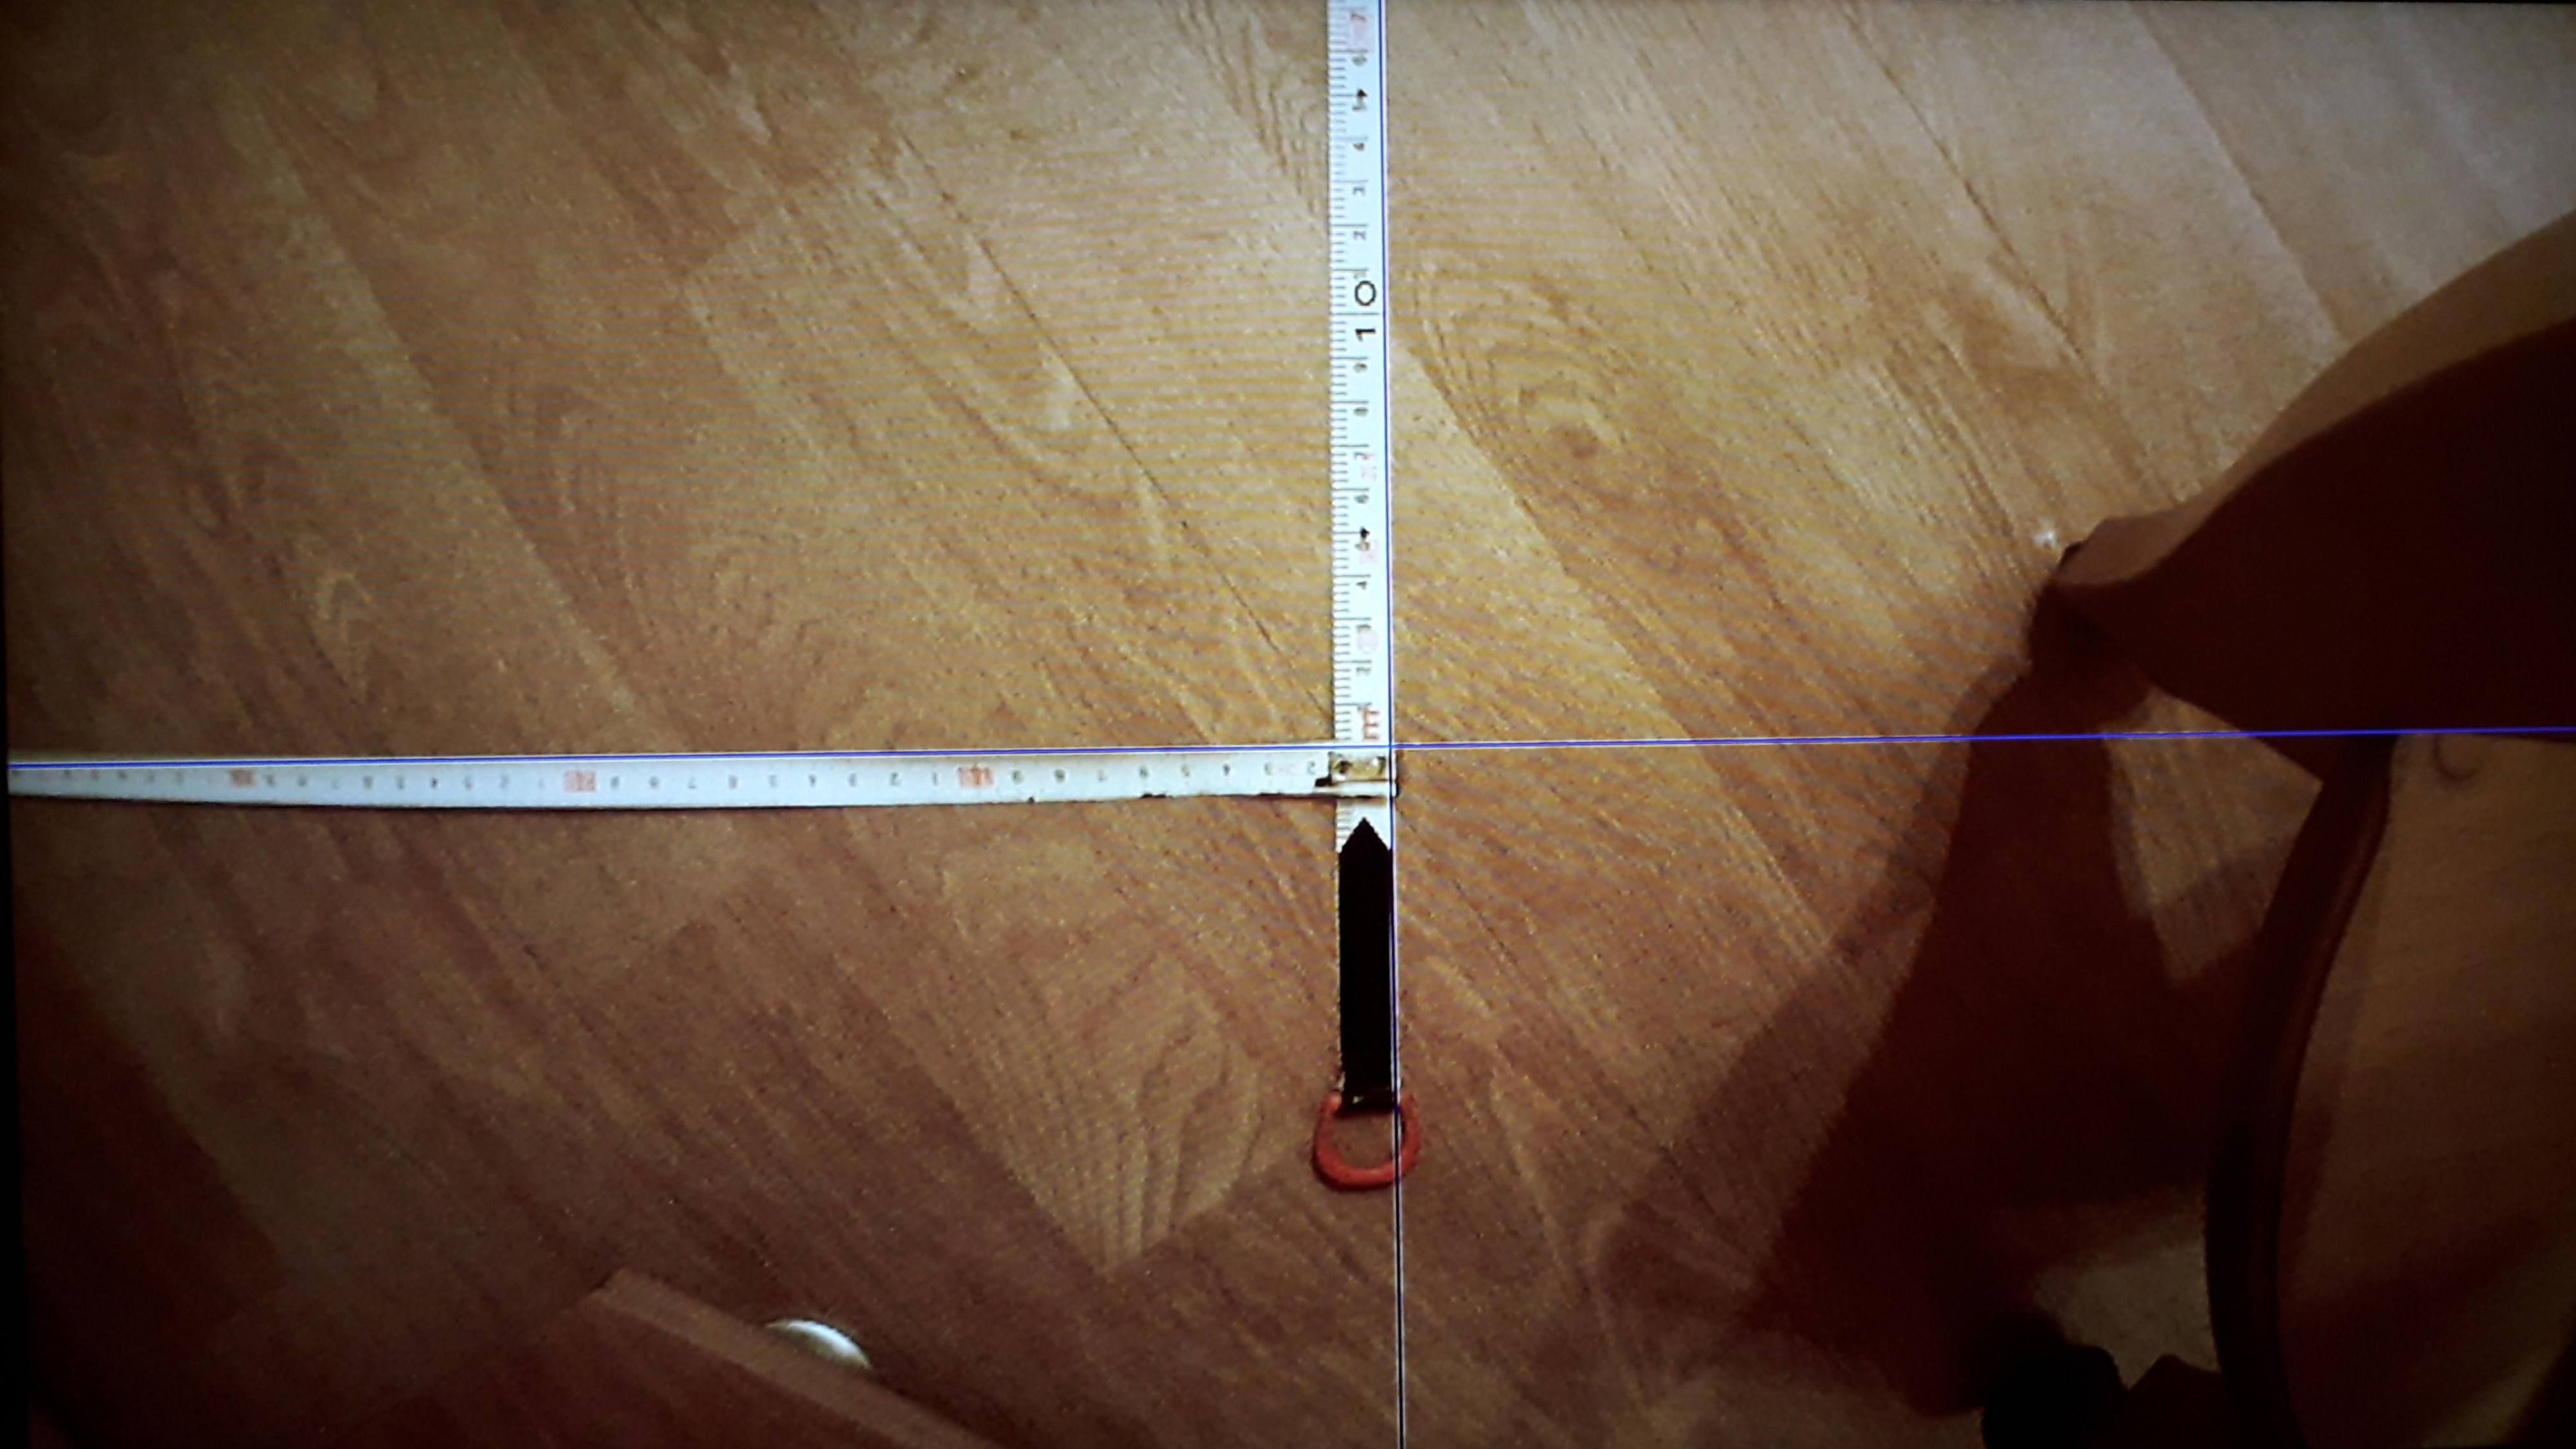
\includegraphics[width=\textwidth]{720p.jpg}
	\caption{Obraz służący do wyznaczenia kąta widzenia kamery dla rozdzielczości 1280 x 720.}
	\label{fig:720p}
\end{figure}

%TODO Jakieś wnioski...


\section{Podsumowanie}

%TODO Kilka zdań o tym modelu...


%TODO2 !!!! Bardzo nie lubię się potwarzać ! I jak dyplomant ignoruje moje uwagi ! To nie może tak być. Tu proszę przekopiować treść rozdziału testy - wybór znacznika i kąta widzenia. Ale nie tylko skopiować, ale też połączyć i uzupełnić zgodnie z uwagami. Natomiast w takim układzie implementacja sprzętowa + te dwa testy (bardziej sprzętowe) do nowego rozdziału (tzn. nowy \chapter). A ten "Test" znika !!!. I stosowana korekta treści we wstępie.



>>>>>>> 1f128f6bdf2d2b222fe828b89fbd544de01b028f
